% Values, gradients, and Hessians.
%%%%%%%%%%%%%%%%%%%%%%%%%%%%%%%%%%

\chapter{Values, gradients, and Hessians} \label{ch: values, gradients, and Hessians}



% Introduction.
%%%%%%%%%%%%%%%

\section{Introduction}


A word of warning before reading this chapter, the topics covered here are quite advanced and are not necessary for understanding how to either use relax or to implement any of the data analysis techniques present within relax.  The material of this chapter is intended as an in-depth explanation of the mathematics involved in the optimisation of the parameters of the model-free models.  As such it contains the chi-squared equation, relaxation equations, spectral density functions, and diffusion tensor equations as well as their gradients (the vector of first partial derivatives) and Hessians (the matrix of second partial derivatives).  All these equations are used in the optimisation of models $m0$ to $m9$; models $tm0$ to $tm9$; the ellipsoidal, spheroidal, and spherical diffusion tensors; and the combination of the diffusion tensor and the model-free models.



% Minimisation concepts.
%%%%%%%%%%%%%%%%%%%%%%%%

\section{Minimisation concepts}
\index{minimisation|textbf}

% The function value.
\subsection{The function value}

At the simplest level all minimisation techniques require at least a function which will supply a single value for different parameter values $\theta$.  For the modelling of NMR relaxation data this function is the chi-squared equation~\eqref{eq: chi-squared} on page~\pageref{eq: chi-squared}.  For certain algorithms, such a simplex minimisation\index{minimisation techniques!simplex}, this single value suffices.


% The gradient.
\subsection{The gradient}

The majority of minimisation algorithms also require the gradient at the point in the space represented by the parameter values $\theta$.  The gradient is a vector of partial derivatives and is defined as
\begin{equation}
 \nabla = \begin{pmatrix}
  \frac{\partial}{\partial \theta_1} \\
  \frac{\partial}{\partial \theta_2} \\
  \vdots \\
  \frac{\partial}{\partial \theta_n} \\
 \end{pmatrix}
\end{equation}

\noindent where $n$ is the total number of parameters in the model.

An example of a powerful algorithm which requires both the value and gradient at current parameter values is the BFGS quasi-Newton minimisation\index{minimisation techniques!BFGS}.  The gradient is also essential for the use of the Method of Multipliers constraints algorithm (also known as the Augmented Lagrangian algorithm).


% The Hessian.
\subsection{The Hessian}

A few optimisation algorithms, which are among the most reliable for model-free analysis, additionally require the Hessian at current parameter values $\theta$.  The Hessian is the matrix of second partial derivatives and is defined as
\begin{equation}
 \nabla^2 = \begin{pmatrix}
  \frac{\partial^2}{{\partial \theta_1}^2}                       & \frac{\partial^2}{\partial \theta_1 \cdot \partial \theta_2}  & \ldots    & \frac{\partial^2}{\partial \theta_1 \cdot \partial \theta_n} \\
  \frac{\partial^2}{\partial \theta_2 \cdot \partial \theta_1} & \frac{\partial^2}{{\partial \theta_2}^2}                        & \ldots    & \frac{\partial^2}{\partial \theta_2 \cdot \partial \theta_n} \\
  \vdots                                                       & \vdots                                                        & \ddots    & \vdots \\
  \frac{\partial^2}{\partial \theta_n \cdot \partial \theta_1} & \frac{\partial^2}{\partial \theta_n \cdot \partial \theta_2}  & \ldots    & \frac{\partial^2}{{\partial \theta_n}^2} \\
 \end{pmatrix}.
\end{equation}

\noindent As the order in which the partial derivatives are calculated is inconsequential the Hessian is symmetric.

The most powerful minimisation algorithm for model-free analysis -- Newton optimisation\index{minimisation techniques!Newton} -- requires the value, gradient, and Hessian at the current parameter values.



% The four parameter combinations.
%%%%%%%%%%%%%%%%%%%%%%%%%%%%%%%%%%

\section{The four parameter combinations}

In model-free analysis four different combinations of parameters can be optimised, each of which requires a different approach to the construction of the chi-squared value, gradient, and Hessian.  These categories depend on whether the model-free parameter set $\Mfset$, the diffusion tensor parameter set $\Diffset$, or both sets are simultaneously optimised.  The addition of the local $\tau_m$ parameter to the model-free set $\Mfset$ creates a fourth parameter combination.




% Optimisation of the model-free models.
%~~~~~~~~~~~~~~~~~~~~~~~~~~~~~~~~~~~~~~~

\subsection{Optimisation of the model-free models}

This is the simplest category as it involves solely the optimisation of the model-free parameters of an individual residue while the diffusion tensor parameters are held constant.  The model-free parameters belong to the set $\Mfset_i$ of the residue $i$.  The models include $m0$ to $m9$ and the dimensionality is low with
\begin{equation}
    \dim \Mfset_i = k \leqslant 5
\end{equation}

\noindent for the most complex model $m8 = \{S^2, \tau_f, S^2_f, \tau_s, R_{ex}\}$.  The relaxation data of a single residue is used to build the chi-squared value, gradient, and Hessian.


% Optimisation of the local tm models.
%~~~~~~~~~~~~~~~~~~~~~~~~~~~~~~~~~~~~~

\subsection{Optimisation of the local $\tau_m$ models}

The addition of the local $\tau_m$ parameter to the set $\Mfset_i$ creates a new set of models which will be labelled $\Localset_i$.  These include models $tm0$ to $tm9$.  The local $\tau_m$ parameter is the single member of the set $\Diffset_i$ and in set notation
\begin{equation}
    \Localset_i = \Diffset_i \cup \Mfset_i.
\end{equation}

Although the Brownian rotational diffusion parameter local $\tau_m$ is optimised, this category is residue specific.  As such the complexity of the optimisation is lower than the next two categories.  It is slightly greater than the optimisation of the set $\Mfset_i$ as
\begin{equation}
    \dim \Localset_i = 1 + k \leqslant 6,
\end{equation}

\noindent where $k$ is the number of model-free parameters.



% Optimisation of the diffusion tensor parameters.
%~~~~~~~~~~~~~~~~~~~~~~~~~~~~~~~~~~~~~~~~~~~~~~~~~

\subsection{Optimisation of the diffusion tensor parameters}

The parameters of the Brownian rotational diffusion tensor belong to the set $\Diffset$.  This set is the union of the geometric parameters $\Diffgeoset = \{\Diff_{iso}, \Diff_a, \Diff_r\}$ and the orientational parameters $\Difforiset$,
\begin{equation}
    \Diffset = \Diffgeoset \cup \Difforiset.
\end{equation}

\noindent When diffusion is spherical solely the geometric parameter $\Diff_{iso}$ is optimised.  When the molecule diffuses as a spheroid the geometric parameters $\Diff_{iso}$ and $\Diff_a$ and the orientational parameters $\theta$ (the polar angle) and $\phi$ (the azimuthal angle) are optimised.  If the molecule diffuses as an ellipsoid the geometric parameters $\Diff_{iso}$, $\Diff_a$, and $\Diff_r$ are optimised together with the Euler angles $\alpha$, $\beta$, and $\gamma$.

This category is defined as the optimisation of solely the parameters of $\Diffset$.  The model-free parameters of $\Mfset$ are held constant.  As all selected residues of the macromolecule are involved in the optimisation, this category is global and can be more complex than the optimisation of $\Mfset_i$ or $\Localset_i$.  The dimensionality of the problem nevertheless low with
\begin{equation}
    \dim \Diffset = 1, \qquad \dim \Diffset = 4, \qquad \dim \Diffset = 6,
\end{equation}

\noindent for the diffusion as a sphere, spheroid, and ellipsoid respectively.



% Optimisation of the global model.
%~~~~~~~~~~~~~~~~~~~~~~~~~~~~~~~~~~

\subsection{Optimisation of the global model $\Space$}

The global model is defined as
\begin{equation}
    \Space = \Diffset \cup \left( \bigcup_{i=1}^l \Mfset_i \right),
\end{equation}

\noindent where $i$ is the residue index and $l$ is the total number of residues used in the analysis.  This is the most complex of the four categories as both diffusion tensor parameters and model-free parameters of all selected residues are optimised simultaneously.  The dimensionality of the model $\Space$ is much greater than the other categories and is equal to
\begin{equation}
    \dim \Space = \dim \Diffset + \sum_{i=1}^l k_i \leqslant 6 + 5l,
\end{equation}

\noindent where $k_i$ is the number of model-free parameters for the residue $i$ and is equal to $\dim \Mfset_i$, the number six corresponds to the maximum dimensionality of $\Diffset$, and the number five corresponds to the maximum dimensionality of $\Mfset_i$.




% Construction of the values, gradients, and Hessians.
%%%%%%%%%%%%%%%%%%%%%%%%%%%%%%%%%%%%%%%%%%%%%%%%%%%%%%

\section{Construction of the values, gradients, and Hessians}


% The sum of chi-squared values.
%~~~~~~~~~~~~~~~~~~~~~~~~~~~~~~~

\subsection{The sum of chi-squared values}

For the single residue models of $\Mfset_i$ and $\Localset_i$ the chi-squared value $\chi^2_i$ which is optimised is simply Equation~\eqref{eq: maths: chi-squared} on page \pageref{eq: maths: chi-squared} in which the relaxation data is that of residue $i$.  However for the global models $\Diffset$ and $\Space$ in which all selected residues are involved the optimised chi-squared value is the sum of those for each residue,
\begin{equation}
    \chi^2 = \sum^l_{i=1} \chi^2_i,
\end{equation}

\noindent where $i$ is the residue index and $l$ is the total number of residues used in the analysis.  This is equivalent to Equation~\eqref{eq: maths: chi-squared} when the index $i$ ranges over the relaxation data of all selected residues.



% Construction of the gradient.
%~~~~~~~~~~~~~~~~~~~~~~~~~~~~~~

\subsection{Construction of the gradient}

% Gradient construction figure.
\begin{figure}
\centerline{\includegraphics[width=0.9\textwidth, bb=143 399 494 777]{images/gradient.eps.gz}}
\caption[The construction of the model-free gradient.]{The construction of the model-free gradient $\nabla \chi^2$ for the global model $\Space$.  For each residue $i$ a different vector $\nabla \chi^2_i$ is constructed.  The first element of the vector represented by the symbol $\partial \Diffset$ (the orange block) is the sub-vector of chi-squared partial derivatives with respect to each of the diffusion tensor parameters $\Diffset_j$.  The rest of the elements, grouped into blocks for each residue denoted by the symbol $\partial \Mfset_i$, are the sub-vectors of chi-squared partial derivatives with respect to each of the model-free parameters $\Mfset_i^j$.  For the residue dependent vector $\nabla \chi^2_i$ the partial derivatives with respect to the model-free parameters of $\Mfset_j$ where $i \ne j$ are zero.  These blocks are left uncoloured.  The complete gradient of $\Space$ is the sum of the vectors $\nabla \chi^2_i$.}\label{fig: gradient construction}
\end{figure}

The construction of the gradient is significantly different for the models $\Mfset_i$, $\Localset_i$, $\Diffset$, and $\Space$.  In Figure~\ref{fig: gradient construction} the construction of the chi-squared gradient $\nabla \chi^2$ for the global model $\Space$ is demonstrated.  In this case
\begin{equation} \label{eq: spaceset gradient}
    \nabla \chi^2 = \sum_{i=1}^l \nabla \chi^2_i,
\end{equation}

\noindent where $\nabla \chi^2_i$ is the vector of partial derivatives of the chi-squared equation $\chi^2_i$ for the residue $i$.  The length of this vector is
\begin{equation}
    \lVert \nabla \chi^2_i \rVert = \dim \Space,
\end{equation}

\noindent with each position of the vector $j$ equal to $\frac{\partial \chi^2_i}{\partial \theta_j}$ where each $\theta_j$ is a parameter of the model.

The construction of the gradient $\nabla \chi^2$ for the model $\Diffset$ is simply a subset of that of $\Space$.  This is demonstrated in Figure~\ref{fig: gradient construction} by simply taking the component of the gradient $\nabla \chi^2_i$ denoted by the symbol $\partial \Diffset$ (the orange blocks) and summing these for all residues.  This sum is given by \eqref{eq: spaceset gradient} and
\begin{equation}
    \lVert \nabla \chi^2_i \rVert = \dim \Diffset.
\end{equation}

For the parameter set $\Localset_i$, which consists of the local $\tau_m$ parameter and the model-free parameters of a single residue, the gradient $\nabla \chi^2_i$ for the residue $i$ is simply the combination of the single orange block and single yellow block of the index $i$ (Figure~\ref{fig: gradient construction}).

The model-free parameter set $\Mfset_i$ is even simpler.  In Figure~\ref{fig: gradient construction} the gradient $\nabla \chi^2_i$ is simply the vector denoted by the single yellow block for the residue $i$.



% Construction of the Hessian.
%~~~~~~~~~~~~~~~~~~~~~~~~~~~~~

\subsection{Construction of the Hessian}

% Hessian kite figure.
\begin{figure}
\centerline{\includegraphics[width=0.8\textwidth, bb=61 11 585 789]{images/kite.eps.gz}}
\caption[The model-free Hessian kite.]{The model-free Hessian kite -- a demonstration of the construction of the model-free Hessian $\nabla^2 \chi^2$ for the global model $\Space$.  For each residue $i$ a different matrix $\nabla^2 \chi^2_i$ is constructed.  The first element of the matrix represented by the two symbols $\partial \Diffset$ (the red block) is the sub-matrix of chi-squared second partial derivatives with respect to the diffusion tensor parameters $\Diffset_j$ and $\Diffset_k$.  The orange blocks are the sub-matrices of chi-squared second partial derivatives with respect to the diffusion parameter $\Diffset_j$ and the model-free parameter $\Mfset_i^k$.  The yellow blocks are the sub-matrices of chi-squared second partial derivatives with respect to the model-free parameters $\Mfset_i^j$ and $\Mfset_i^k$.  For the residue dependent matrix $\nabla^2 \chi^2_i$ the second partial derivatives with respect to the model-free parameters $\Mfset_l^j$ and $\Mfset_l^k$ where $i \ne l$ are zero.  In addition, the second partial derivatives with respect to the model-free parameters $\Mfset_i^j$ and $\Mfset_l^k$ where $i \ne l$ are also zero.  These blocks of sub-matrices are left uncoloured.  The complete Hessian of $\Space$ is the sum of the matrices $\nabla^2 \chi^2_i$.}\label{fig: Hessian kite}
\end{figure}

The construction of the Hessian for the models $\Mfset_i$, $\Localset_i$, $\Diffset$, and $\Space$ is very similar to the procedure used for the gradient.  The chi-squared Hessian for the global models $\Diffset$ and $\Space$ is
\begin{equation} \label{eq: spaceset Hessian}
    \nabla^2 \chi^2 = \sum_{i=1}^l \nabla^2 \chi^2_i.
\end{equation}

\noindent Figure~\ref{fig: Hessian kite} demonstrates the construction of the full Hessian for the model $\Space$.  The Hessian for the model $\Diffset$ is the sum of all the red blocks.  The Hessian for the model $\Localset_i$ is the combination of the single red block for residue $i$, the two orange blocks representing the sub-matrices of chi-squared second partial derivatives with respect to the diffusion parameter $\Diffset_j$ and the model-free parameter $\Mfset_i^k$, and the single yellow block for that residue.  The Hessian for the model-free model $\Mfset_i$ is simply the sub-matrix for the residue $i$ coloured yellow.



% The value, gradient, and Hessian dependency chain.
%%%%%%%%%%%%%%%%%%%%%%%%%%%%%%%%%%%%%%%%%%%%%%%%%%%%

\section{The value, gradient, and Hessian dependency chain}

The dependency chain which was outlined in the model-free chapter -- that the chi-squared function is dependent on the transformed relaxation equations which are dependent on the relaxation equations which themselves are dependent on the spectral density functions -- combine with the values, gradients, and Hessians to create a complex web of dependencies.  The relationship between all the values, gradients, and Hessians are outlined in Figure~\ref{fig: dependencies}.

% Dependency figure.
\begin{figure}
\centerline{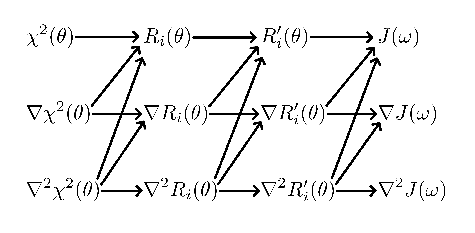
\includegraphics[width=0.8\textwidth, bb=14 14 226 110]{images/dependencies.eps.gz}}
\caption[$\chi^2$ dependencies of the values, gradients, and Hessians.]{Dependencies between the $\chi^2$, transformed relaxation, relaxation, and spectral density equations, gradients, and Hessians.}\label{fig: dependencies}
\end{figure}



% The chi-squared value, gradient, and Hessian.
%%%%%%%%%%%%%%%%%%%%%%%%%%%%%%%%%%%%%%%%%%%%%%%

\section{The $\chi^2$ value, gradient, and Hessian}

% The chi-squared value.
\subsection{The $\chi^2$ value}

As was presented in Equation~\eqref{eq: chi-squared} on page~\pageref{eq: chi-squared} the $\chi^2$ value is
\begin{equation} \label{eq: maths: chi-squared}
 \chi^2(\theta) = \sum_{i=1}^n \frac{(\Ri - \Ri(\theta))^2}{\sigma_i^2},
\end{equation}

\noindent where the summation index $i$ ranges over all the relaxation data of all residues used in the analysis.



% The chi-squared gradient.
\subsection{The $\chi^2$ gradient}

The $\chi^2$ gradient in vector notation is
\begin{equation}
 \nabla \chi^2(\theta) = 2 \sum_{i=1}^n \frac{(\Ri - \Ri(\theta))^2}{\sigma_i^2} \nabla \Ri(\theta).
\end{equation}



% The chi-squared Hessian.
\subsection{The $\chi^2$ Hessian}

The $\chi^2$ Hessian in vector notation is
\begin{equation}
 \nabla^2 \chi^2(\theta) = 2 \sum_{i=1}^n \frac{1}{\sigma_i^2} \left(\nabla \Ri(\theta) \cdot \nabla \Ri(\theta)^T - (\Ri - \Ri(\theta)) \nabla^2 \Ri(\theta) \right).
\end{equation}



% The Ri values, gradients, and Hessians.
%%%%%%%%%%%%%%%%%%%%%%%%%%%%%%%%%%%%%%%%%

\newpage
\section{The $\Ri(\theta)$ values, gradients, and Hessians}


% The Ri values.
\subsection{The $\Ri(\theta)$ values}

The $\Ri(\theta)$ values are given by
\begin{subequations}
\begin{align}
    \Rone(\theta) & = \Rone'(\theta), \label{eq: Ri trans: R1} \\
    \Rtwo(\theta) & = \Rtwo'(\theta), \label{eq: Ri trans: R2} \\
    \mathrm{NOE}(\theta) & = 1 + \frac{\gH}{\gX} \frac{\crossrate(\theta)}{\Rone(\theta)}. \label{eq: Ri trans: NOE}
\end{align}
\end{subequations}


% The Ri gradients.
\subsection{The $\Ri(\theta)$ gradients}

The $\Ri(\theta)$ gradients in vector notation are
\begin{subequations}
\begin{align}
    \nabla \Rone(\theta) & = \nabla \Rone'(\theta), \label{eq: Ri trans: dR1} \\
    \nabla \Rtwo(\theta) & = \nabla \Rtwo'(\theta), \label{eq: Ri trans: dR2} \\
    \nabla \mathrm{NOE}(\theta) & = \frac{\gH}{\gX} \frac{1}{\Rone(\theta)^2} \Big(
        \Rone(\theta) \nabla \crossrate(\theta) - \crossrate(\theta) \nabla \Rone(\theta)
    \Big). \label{eq: Ri trans: dNOE}
\end{align}
\end{subequations}


% The Ri Hessians.
\subsection{The $\Ri(\theta)$ Hessians}

The $\Ri(\theta)$ Hessians in vector notation are
\begin{subequations}
\begin{align}
    \nabla^2 \Rone(\theta) & = \nabla^2 \Rone'(\theta), \label{eq: Ri trans: d2R1} \\
    \nabla^2 \Rtwo(\theta) & = \nabla^2 \Rtwo'(\theta), \label{eq: Ri trans: d2R2} \\
    \nabla^2 \mathrm{NOE}(\theta) & = \frac{\gH}{\gX} \frac{1}{\Rone(\theta)^3} \bigg[
        \crossrate(\theta) \Big( 2 \nabla \Rone(\theta) \cdot \nabla \Rone(\theta)^T - \Rone(\theta) \nabla^2 \Rone(\theta) \Big) \nonumber\\
        & \quad - \Rone(\theta) \Big( \nabla \crossrate(\theta) \cdot \nabla \Rone(\theta)^T - \Rone(\theta) \nabla^2 \crossrate(\theta) \Big)
    \bigg]. \label{eq: Ri trans: d2NOE}
\end{align}
\end{subequations}



% Ri' values, gradients, and Hessians.
%%%%%%%%%%%%%%%%%%%%%%%%%%%%%%%%%%%%%%

\newpage
\section{$\Ri'(\theta)$ values, gradients, and Hessians}

The partial and second partial derivatives of the relaxation equations of the set R$'(\theta)$ are different for each parameter of the vector $\theta$.  The vector representation of the gradient $\nabla \textrm{R}_i'(\theta)$ and the matrix representation of the Hessian $\nabla^2 \textrm{R}_i'(\theta)$ can be reconstructed from the individual elements presented in the next section.


% Components.
%~~~~~~~~~~~~

\subsection{Components of the $\Ri'(\theta)$ equations}

To simplify the calculations of the gradients and Hessians the $\Ri'(\theta)$ equations have been broken down into a number of components.  These include the dipolar and CSA constants as well as the dipolar and CSA spectral density terms for each of the three transformed relaxation data types \{$\Rone$, $\Rtwo$, $\crossrate$\}.  The segregation of these components simplifies the maths as many partial derivatives of the components are zero.


% Dipolar comps.
\subsubsection{Dipolar constant}

The dipolar constant is defined as
\begin{equation}
    d = \frac{1}{4} \left(\frac{\mu_0}{4\pi}\right)^2 \frac{\left( \gH \gX \hbar \right)^2}{<r^6>}. \label{eq: Ri': d}
\end{equation}

\noindent This component of the relaxation equations is independent of the parameter of the spectral density function $\theta_j$, the chemical exchange parameter $\rho_{ex}$, and the CSA parameter $\Delta\sigma$.  Therefore the partial and second partial derivatives with respect to these parameters is zero.  Only the derivative with respect to the bond length $r$ is non-zero being
\begin{equation}
    d' \equiv \frac{\mathrm{d} d}{\mathrm{d} r} = - \frac{3}{2} \left(\frac{\mu_0}{4\pi}\right)^2 \frac{\left( \gH \gX \hbar \right)^2}{<r^7>}. \label{eq: Ri': d'}
\end{equation}

\noindent The second derivative with respect to the bond length is
\begin{equation}
    d'' \equiv \frac{\mathrm{d}^2 d}{\mathrm{d} r^2} = \frac{21}{2} \left(\frac{\mu_0}{4\pi}\right)^2 \frac{\left( \gH \gX \hbar \right)^2}{<r^8>}. \label{eq: Ri': d"}
\end{equation}


% CSA comps.
\subsubsection{CSA constant}

The CSA constant is defined as
\begin{equation}
    c = \frac{\left(\omega_X \cdot \Delta\sigma \right)^2}{3}. \label{eq: Ri': c}
\end{equation}

\noindent The partial derivative of this component with respect to all parameters but the CSA parameter $\Delta\sigma$ is zero.  This derivative is
\begin{equation}
    c' \equiv \frac{\mathrm{d} c}{\mathrm{d} \Delta\sigma} = \frac{2 \omega_X^2 \cdot \Delta\sigma}{3}. \label{eq: Ri': c'}
\end{equation}

\noindent The CSA constant second derivative with respect to $\Delta\sigma$ is
\begin{equation}
    c'' \equiv \frac{\mathrm{d}^2 c}{\mathrm{d} \Delta\sigma^2} = \frac{2 \omega_X^2}{3}. \label{eq: Ri': c"}
\end{equation}


% Rex comps.
\subsubsection{$R_{ex}$ constant}

The $R_{ex}$ constant is defined as
\begin{equation}
    R_{ex} = \rho_{ex} (2 \pi \omega_H)^2 . \label{eq: Ri': Rex}
\end{equation}

\noindent The partial derivative of this component with respect to all parameters but the chemical exchange parameter $\rho_{ex}$ is zero.  This derivative is
\begin{equation}
    R_{ex}' \equiv \frac{\mathrm{d} R_{ex}}{\mathrm{d} \rho_{ex}} = (2 \pi \omega_H)^2. \label{eq: Ri': Rex'}
\end{equation}

\noindent The $R_{ex}$ constant second derivative with respect to $\rho_{ex}$ is
\begin{equation}
    R_{ex}'' \equiv \frac{\mathrm{d}^2 R_{ex}}{\mathrm{d} \rho_{ex}^2} = 0. \label{eq: Ri': Rex"}
\end{equation}


% R1 dip Spectral density terms.
\subsubsection{Spectral density terms of the $\Rone$ dipolar component}

For the dipolar component of the $\Rone$ equation~\eqref{eq: R1} on page~\pageref{eq: R1} the spectral density terms are
\begin{equation}
    J_d^{\Rone} = J(\omega_H - \omega_X) + 3J(\omega_X) + 6J(\omega_H + \omega_X).  \label{eq: J terms: JR1d}
\end{equation}

\noindent The partial derivative of these terms with respect to the spectral density function parameter $\theta_j$ is
\begin{equation}
    {J_d^{\Rone}}' \equiv \frac{\partial J_d^{\Rone}}{\partial \theta_j}
        = \frac{\partial J(\omega_H - \omega_X)}{\partial \theta_j}
        + 3 \frac{\partial J(\omega_X)}{\partial \theta_j}
        + 6 \frac{\partial J(\omega_H + \omega_X)}{\partial \theta_j}.  \label{eq: J terms: JR1d'}
\end{equation}

\noindent The second partial derivative with respect to the spectral density function parameters $\theta_j$ and $\theta_k$ is
\begin{equation}
    {J_d^{\Rone}}'' \equiv \frac{\partial^2 J_d^{\Rone}}{\partial \theta_j \cdot \partial \theta_k}
        = \frac{\partial^2 J(\omega_H - \omega_X)}{\partial \theta_j \cdot \partial \theta_k}
        + 3 \frac{\partial^2 J(\omega_X)}{\partial \theta_j \cdot \partial \theta_k}
        + 6 \frac{\partial^2 J(\omega_H + \omega_X)}{\partial \theta_j \cdot \partial \theta_k}.  \label{eq: J terms: JR1d"}
\end{equation}


% R1 CSA Spectral density terms.
\subsubsection{Spectral density terms of the $\Rone$ CSA component}

For the CSA component of the $\Rone$ equation~\eqref{eq: R1} on page~\pageref{eq: R1} the spectral density terms are
\begin{equation}
    J_c^{\Rone} = J(\omega_X).  \label{eq: J terms: JR1c}
\end{equation}

\noindent The partial derivative of these terms with respect to the spectral density function parameter $\theta_j$ is
\begin{equation}
    {J_c^{\Rone}}' \equiv \frac{\partial J_c^{\Rone}}{\partial \theta_j}
        = \frac{\partial J(\omega_X)}{\partial \theta_j}.  \label{eq: J terms: JR1c'}
\end{equation}

\noindent The second partial derivative with respect to the spectral density function parameters $\theta_j$ and $\theta_k$ is
\begin{equation}
    {J_c^{\Rone}}'' \equiv \frac{\partial^2 J_c^{\Rone}}{\partial \theta_j . \partial \theta_k}
        = \frac{\partial^2 J(\omega_X)}{\partial \theta_j \cdot \partial \theta_k}.  \label{eq: J terms: JR1c"}
\end{equation}


% R2 dip Spectral density terms.
\subsubsection{Spectral density terms of the $\Rtwo$ dipolar component}

For the dipolar component of the $\Rtwo$ equation~\eqref{eq: R2} on page~\pageref{eq: R2} the spectral density terms are
\begin{equation}
    J_d^{\Rtwo} = 4J(0) + J(\omega_H - \omega_X) + 3J(\omega_X) + 6J(\omega_H) + 6J(\omega_H + \omega_X).  \label{eq: J terms: JR2d}
\end{equation}

\noindent The partial derivative of these terms with respect to the spectral density function parameter $\theta_j$ is
\begin{equation}
    {J_d^{\Rtwo}}' \equiv \frac{\partial J_d^{\Rtwo}}{\partial \theta_j}
        = 4 \frac{\partial J(0)}{\partial \theta_j}
        + \frac{\partial J(\omega_H - \omega_X)}{\partial \theta_j}
        + 3 \frac{\partial J(\omega_X)}{\partial \theta_j}
        + 6 \frac{\partial J(\omega_H)}{\partial \theta_j}
        + 6 \frac{\partial J(\omega_H + \omega_X)}{\partial \theta_j}.  \label{eq: J terms: JR2d'}
\end{equation}

\noindent The second partial derivative with respect to the spectral density function parameters $\theta_j$ and $\theta_k$ is
\begin{multline}
    {J_d^{\Rtwo}}'' \equiv \frac{\partial^2 J_d^{\Rtwo}}{\partial \theta_j \cdot \partial \theta_k}
        = 4 \frac{\partial^2 J(0)}{\partial \theta_j \cdot \partial \theta_k}
        + \frac{\partial^2 J(\omega_H - \omega_X)}{\partial \theta_j \cdot \partial \theta_k}
        + 3 \frac{\partial^2 J(\omega_X)}{\partial \theta_j \cdot \partial \theta_k} \\
        + 6 \frac{\partial^2 J(\omega_H)}{\partial \theta_j \cdot \partial \theta_k}
        + 6 \frac{\partial^2 J(\omega_H + \omega_X)}{\partial \theta_j \cdot \partial \theta_k}.  \label{eq: J terms: JR2d"}
\end{multline}


% R2 CSA Spectral density terms.
\subsubsection{Spectral density terms of the $\Rtwo$ CSA component}

For the CSA component of the $\Rtwo$ equation~\eqref{eq: R2} on page~\pageref{eq: R2} the spectral density terms are
\begin{equation}
    J_c^{\Rtwo} = 4J(0) + 3J(\omega_X).  \label{eq: J terms: JR2c}
\end{equation}

\noindent The partial derivative of these terms with respect to the spectral density function parameter $\theta_j$ is
\begin{equation}
    {J_c^{\Rtwo}}' \equiv \frac{\partial J_c^{\Rtwo}}{\partial \theta_j}
        = 4 \frac{\partial J(0)}{\partial \theta_j}
        + 3 \frac{\partial J(\omega_X)}{\partial \theta_j}.  \label{eq: J terms: JR2c'}
\end{equation}

\noindent The second partial derivative with respect to the spectral density function parameters $\theta_j$ and $\theta_k$ is
\begin{equation}
    {J_c^{\Rtwo}}'' \equiv \frac{\partial^2 J_c^{\Rtwo}}{\partial \theta_j \cdot \partial \theta_k}
        = 4 \frac{\partial^2 J(0)}{\partial \theta_j \cdot \partial \theta_k}
        + 3 \frac{\partial^2 J(\omega_X)}{\partial \theta_j \cdot \partial \theta_k}.  \label{eq: J terms: JR2c"}
\end{equation}


% Sigma_NOE dip Spectral density terms.
\subsubsection{Spectral density terms of the $\crossrate$ dipolar component}

For the dipolar component of the $\crossrate$ equation~\eqref{eq: sigma_NOE} on page~\pageref{eq: sigma_NOE} the spectral density terms are
\begin{equation}
    J_d^{\crossrate} = 6J(\omega_H + \omega_X) - J(\omega_H - \omega_X).  \label{eq: J terms: JsigmaNOEd}
\end{equation}

\noindent The partial derivative of these terms with respect to the spectral density function parameter $\theta_j$ is
\begin{equation}
    {J_d^{\crossrate}}' \equiv \frac{\partial J_d^{\crossrate}}{\partial \theta_j}
        = 6 \frac{\partial J(\omega_H + \omega_X)}{\partial \theta_j}
          - \frac{\partial J(\omega_H - \omega_X)}{\partial \theta_j}.  \label{eq: J terms: JsigmaNOEd'}
\end{equation}

\noindent The second partial derivative with respect to the spectral density function parameters $\theta_j$ and $\theta_k$ is
\begin{equation}
    {J_d^{\crossrate}}'' \equiv \frac{\partial^2 J_d^{\crossrate}}{\partial \theta_j \cdot \partial \theta_k}
        = 6 \frac{\partial^2 J(\omega_H + \omega_X)}{\partial \theta_j \cdot \partial \theta_k}
          - \frac{\partial^2 J(\omega_H - \omega_X)}{\partial \theta_j \cdot \partial \theta_k}.  \label{eq: J terms: JsigmaNOEd"}
\end{equation}



% Ri' values.
%~~~~~~~~~~~~

\subsection{$\Ri'(\theta)$ values}

Using the components of the relaxation equations defined above the three relaxation equations can be re-expressed as
\begin{subequations}
\begin{align}
    \Rone(\theta) & = d J_d^{\Rone} + c J_c^{\Rone},                          \label{eq: Ri': R1} \\
    \Rtwo(\theta) & = \frac{d}{2} J_d^{\Rtwo} + \frac{c}{6} J_c^{\Rtwo},      \label{eq: Ri': R2} \\
    \crossrate(\theta) & = d J_d^{\crossrate}.                          \label{eq: Ri': sigmaNOE}
\end{align}
\end{subequations}



% Ri' gradients.
%~~~~~~~~~~~~~~~

\subsection{$\Ri'(\theta)$ gradients}

A different partial derivative exists for the spectral density function parameter $\theta_j$, the chemical exchange parameter $\rho_{ex}$, CSA parameter $\Delta\sigma$, and bond length parameter $r$.  In model-free analysis the spectral density parameters include both the parameters of the diffusion tensor and the parameters of the various model-free models.


% Spectral density function parameter.
\subsubsection{$\theta_j$ partial derivative}

The partial derivatives of the relaxation equations with respect to the spectral density function parameter $\theta_j$ are
\begin{subequations}
\begin{align}
    \frac{\partial \Rone(\theta)}{\partial \theta_j} &= d {J_d^{\Rone}}' + c {J_c^{\Rone}}',                      \label{eq: Ri': dR1/dmf} \\
    \frac{\partial \Rtwo(\theta)}{\partial \theta_j} &= \frac{d}{2} {J_d^{\Rtwo}}' + \frac{c}{6} {J_c^{\Rtwo}}',  \label{eq: Ri': dR2/dmf} \\
    \frac{\partial \crossrate(\theta)}{\partial \theta_j} &= d {J_d^{\crossrate}}'.                         \label{eq: Ri': dsigmaNOE/dmf}
\end{align}
\end{subequations}


% Chemical exchange parameter.
\subsubsection{$\rho_{ex}$ partial derivative}

The partial derivatives of the relaxation equations with respect to the chemical exchange parameter $\rho_{ex}$ are
\begin{subequations}
\begin{align}
    \frac{\partial \Rone(\theta)}{\partial \rho_{ex}} &= 0,          \label{eq: Ri': dR1/dRex} \\
    \frac{\partial \Rtwo(\theta)}{\partial \rho_{ex}} &= (2 \pi \omega_H)^2,          \label{eq: Ri': dR2/dRex} \\
    \frac{\partial \crossrate(\theta)}{\partial \rho_{ex}} &= 0.   \label{eq: Ri': dsigmaNOE/dRex}
\end{align}
\end{subequations}


% CSA parameter.
\subsubsection{$\Delta\sigma$ partial derivative}

The partial derivatives of the relaxation equations with respect to the CSA parameter $\Delta\sigma$ are
\begin{subequations}
\begin{align}
    \frac{\partial \Rone(\theta)}{\partial \Delta\sigma} &= c' J_c^{\Rone},             \label{eq: Ri': dR1/dCSA} \\
    \frac{\partial \Rtwo(\theta)}{\partial \Delta\sigma} &= \frac{c'}{6} J_c^{\Rtwo},   \label{eq: Ri': dR2/dCSA} \\
    \frac{\partial \crossrate(\theta)}{\partial \Delta\sigma} &= 0.                 \label{eq: Ri': dsigmaNOE/dCSA}
\end{align}
\end{subequations}


% Bond length parameter.
\subsubsection{$r$ partial derivative}

The partial derivatives of the relaxation equations with respect to the bond length parameter $r$ are
\begin{subequations}
\begin{align}
    \frac{\partial \Rone(\theta)}{\partial r} &= d' J_d^{\Rone},                \label{eq: Ri': dR1/dr} \\
    \frac{\partial \Rtwo(\theta)}{\partial r} &= \frac{d'}{2} J_d^{\Rtwo},      \label{eq: Ri': dR2/dr} \\
    \frac{\partial \crossrate(\theta)}{\partial r} &= d' J_d^{\crossrate}.  \label{eq: Ri': dsigmaNOE/dr}
\end{align}
\end{subequations}



% Ri' Hessians.
%~~~~~~~~~~~~~~

\subsection{$\Ri'(\theta)$ Hessians}

Again different second partial derivatives with respect to the spectral density function parameters $\theta_j$ and $\theta_k$, the chemical exchange parameter $\rho_{ex}$, CSA parameter $\Delta\sigma$, and bond length parameter $r$.  These second partial derivatives are the components of the $\Ri'(\theta)$ Hessian matrices.


% Spectral density function parameter -- Spectral density function parameter.
\subsubsection{$\theta_j$ -- $\theta_k$ partial derivative}

The second partial derivatives of the relaxation equations with respect to the spectral density function parameters $\theta_j$ and $\theta_k$ are
\begin{subequations}
\begin{align}
    \frac{\partial^2 \Rone(\theta)}{\partial \theta_j \cdot \partial \theta_k} &= d {J_d^{\Rone}}'' + c {J_c^{\Rone}}'',                      \label{eq: Ri': d2R1/dmfj.dmfk} \\
    \frac{\partial^2 \Rtwo(\theta)}{\partial \theta_j \cdot \partial \theta_k} &= \frac{d}{2} {J_d^{\Rtwo}}'' + \frac{c}{6} {J_c^{\Rtwo}}'',  \label{eq: Ri': d2R2/dmfj.dmfk} \\
    \frac{\partial^2 \crossrate(\theta)}{\partial \theta_j \cdot \partial \theta_k} &= d {J_d^{\crossrate}}''.                          \label{eq: Ri': d2sigmaNOE/dmfj.dmfk}
\end{align}
\end{subequations}


% Spectral density function parameter -- Chemical exchange parameter.
\subsubsection{$\theta_j$ -- $\rho_{ex}$ partial derivative}

The second partial derivatives of the relaxation equations with respect to the spectral density function parameter $\theta_j$ and the chemical exchange parameter $\rho_{ex}$ are
\begin{subequations}
\begin{align}
    \frac{\partial^2 \Rone(\theta)}{\partial \theta_j \cdot \partial \rho_{ex}} &= 0,        \label{eq: Ri': d2R1/dmfj.dRex} \\
    \frac{\partial^2 \Rtwo(\theta)}{\partial \theta_j \cdot \partial \rho_{ex}} &= 0,        \label{eq: Ri': d2R2/dmfj.dRex} \\
    \frac{\partial^2 \crossrate(\theta)}{\partial \theta_j \cdot \partial \rho_{ex}} &= 0. \label{eq: Ri': d2sigmaNOE/dmfj.dRex}
\end{align}
\end{subequations}


% Spectral density function parameter -- CSA parameter.
\subsubsection{$\theta_j$ -- $\Delta\sigma$ partial derivative}

The second partial derivatives of the relaxation equations with respect to the spectral density function parameter $\theta_j$ and the CSA parameter $\Delta\sigma$ are
\begin{subequations}
\begin{align}
    \frac{\partial^2 \Rone(\theta)}{\partial \theta_j \cdot \partial \Delta\sigma} &= c' {J_c^{\Rone}}',            \label{eq: Ri': d2R1/dmfj.dCSA} \\
    \frac{\partial^2 \Rtwo(\theta)}{\partial \theta_j \cdot \partial \Delta\sigma} &= \frac{c'}{6} {J_c^{\Rtwo}}',  \label{eq: Ri': d2R2/dmfj.dCSA} \\
    \frac{\partial^2 \crossrate(\theta)}{\partial \theta_j \cdot \partial \Delta\sigma} &= 0.                   \label{eq: Ri': d2sigmaNOE/dmfj.dCSA}
\end{align}
\end{subequations}


% Spectral density function parameter -- Bond length parameter.
\subsubsection{$\theta_j$ -- $r$ partial derivative}

The second partial derivatives of the relaxation equations with respect to the spectral density function parameter $\theta_j$ and the bond length parameter $r$ are
\begin{subequations}
\begin{align}
    \frac{\partial^2 \Rone(\theta)}{\partial \theta_j \cdot \partial r} &= d' {J_d^{\Rone}}',               \label{eq: Ri': d2R1/dmfj.dr} \\
    \frac{\partial^2 \Rtwo(\theta)}{\partial \theta_j \cdot \partial r} &= \frac{d'}{2} {J_d^{\Rtwo}}',     \label{eq: Ri': d2R2/dmfj.dr} \\
    \frac{\partial^2 \crossrate(\theta)}{\partial \theta_j \cdot \partial r} &= d' {J_d^{\crossrate}}'. \label{eq: Ri': d2sigmaNOE/dmfj.dr}
\end{align}
\end{subequations}


% Chemical exchange parameter -- Chemical exchange parameter.
\subsubsection{$\rho_{ex}$ -- $\rho_{ex}$ partial derivative}

The second partial derivatives of the relaxation equations with respect to the chemical exchange parameter $\rho_{ex}$ twice are
\begin{subequations}
\begin{align}
    \frac{\partial^2 \Rone(\theta)}{{\partial \rho_{ex}}^2} &= 0,        \label{eq: Ri': d2R1/dRex2} \\
    \frac{\partial^2 \Rtwo(\theta)}{{\partial \rho_{ex}}^2} &= 0,        \label{eq: Ri': d2R2/dRex2} \\
    \frac{\partial^2 \crossrate(\theta)}{{\partial \rho_{ex}}^2} &= 0. \label{eq: Ri': d2sigmaNOE/dRex2}
\end{align}
\end{subequations}


% Chemical exchange parameter -- CSA parameter.
\subsubsection{$\rho_{ex}$ -- $\Delta\sigma$ partial derivative}

The second partial derivatives of the relaxation equations with respect to the chemical exchange parameter $\rho_{ex}$ and the CSA parameter $\Delta\sigma$ are
\begin{subequations}
\begin{align}
    \frac{\partial^2 \Rone(\theta)}{\partial \rho_{ex} \cdot \partial \Delta\sigma} &= 0,        \label{eq: Ri': d2R1/dRex.dCSA} \\
    \frac{\partial^2 \Rtwo(\theta)}{\partial \rho_{ex} \cdot \partial \Delta\sigma} &= 0,        \label{eq: Ri': d2R2/dRex.dCSA} \\
    \frac{\partial^2 \crossrate(\theta)}{\partial \rho_{ex} \cdot \partial \Delta\sigma} &= 0. \label{eq: Ri': d2sigmaNOE/dRex.dCSA}
\end{align}
\end{subequations}


% Chemical exchange parameter -- Bond length parameter.
\subsubsection{$\rho_{ex}$ -- $r$ partial derivative}

The second partial derivatives of the relaxation equations with respect to the chemical exchange parameter $\rho_{ex}$ and the bond length parameter $r$ are
\begin{subequations}
\begin{align}
    \frac{\partial^2 \Rone(\theta)}{\partial \rho_{ex} \cdot \partial r} &= 0,           \label{eq: Ri': d2R1/dRex.dr} \\
    \frac{\partial^2 \Rtwo(\theta)}{\partial \rho_{ex} \cdot \partial r} &= 0,           \label{eq: Ri': d2R2/dRex.dr} \\
    \frac{\partial^2 \crossrate(\theta)}{\partial \rho_{ex} \cdot \partial r} &= 0.    \label{eq: Ri': d2sigmaNOE/dRex.dr}
\end{align}
\end{subequations}


% CSA parameter -- CSA parameter.
\subsubsection{$\Delta\sigma$ -- $\Delta\sigma$ partial derivative}

The second partial derivatives of the relaxation equations with respect to the CSA parameter $\Delta\sigma$ twice are
\begin{subequations}
\begin{align}
    \frac{\partial^2 \Rone(\theta)}{{\partial \Delta\sigma}^2} &= c'' J_c^{\Rone},              \label{eq: Ri': d2R1/dCSA2} \\
    \frac{\partial^2 \Rtwo(\theta)}{{\partial \Delta\sigma}^2} &= \frac{c''}{6} J_c^{\Rtwo},    \label{eq: Ri': d2R2/dCSA2} \\
    \frac{\partial^2 \crossrate(\theta)}{{\partial \Delta\sigma}^2} &= 0.                   \label{eq: Ri': d2sigmaNOE/dCSA2}
\end{align}
\end{subequations}


% CSA parameter -- Bond length parameter.
\subsubsection{$\Delta\sigma$ -- $r$ partial derivative}

The second partial derivatives of the relaxation equations with respect to the CSA parameter $\Delta\sigma$ and the bond length parameter $r$ are
\begin{subequations}
\begin{align}
    \frac{\partial^2 \Rone(\theta)}{\partial \Delta\sigma \cdot \partial r} &= 0,         \label{eq: Ri': d2R1/dCSA.dr} \\
    \frac{\partial^2 \Rtwo(\theta)}{\partial \Delta\sigma \cdot \partial r} &= 0,         \label{eq: Ri': d2R2/dCSA.dr} \\
    \frac{\partial^2 \crossrate(\theta)}{\partial \Delta\sigma \cdot \partial r} &= 0.  \label{eq: Ri': d2sigmaNOE/dCSA.dr}
\end{align}
\end{subequations}


% Bond length parameter -- Bond length parameter.
\subsubsection{$r$ -- $r$ partial derivative}

The second partial derivatives of the relaxation equations with respect to the bond length parameter $r$ twice are
\begin{subequations}
\begin{align}
    \frac{\partial^2 \Rone(\theta)}{{\partial r}^2} &= d'' J_d^{\Rone},                 \label{eq: Ri': d2R1/dr2} \\
    \frac{\partial^2 \Rtwo(\theta)}{{\partial r}^2} &= \frac{d''}{2} J_d^{\Rtwo},       \label{eq: Ri': d2R2/dr2} \\
    \frac{\partial^2 \crossrate(\theta)}{{\partial r}^2} &= d'' J_d^{\crossrate}.   \label{eq: Ri': d2sigmaNOE/dr2}
\end{align}
\end{subequations}




% Model-free analysis.
%%%%%%%%%%%%%%%%%%%%%%

\newpage
\section{Model-free analysis}



% The model-free equations.
%~~~~~~~~~~~~~~~~~~~~~~~~~~

\subsection{The model-free equations}

In the original model-free analysis of \cite{LipariSzabo82a} the correlation function $C(\tau)$ of the XH bond vector is approximated by decoupling the internal fluctuations of the bond vector $C_\mathrm{I}(\tau)$ from the correlation function of the overall Brownian rotational diffusion $C_\mathrm{O}(\tau)$ by the equation
\begin{equation}
    C(\tau) = C_\mathrm{O}(\tau) \cdot C_\mathrm{I}(\tau).
\end{equation}

\noindent The overall correlation functions of the diffusion of a sphere, spheroid, and ellipsoid are presented respectively in section~\ref{ellipsoid equation} on page~\pageref{ellipsoid equation}, section~\ref{spheroid equation} on page~\pageref{spheroid equation}, and section~\ref{sphere equation} on page~\pageref{sphere equation}.  These three different equations can be combined into one generic correlation function which is independent of the type of diffusion.  This generic correlation function is
\begin{equation}
    C_\mathrm{O}(\tau) = \frac{1}{5} \sum_{i=-k}^k c_i \cdot e^{-\tau/\tau_i},
\end{equation}

\noindent where $c_i$ are the weights and $\tau_i$ are correlation times of the exponential terms.  In the original model-free analysis of \citet{LipariSzabo82a,LipariSzabo82b} the internal motions are modelled by the correlation function
\begin{equation}
    C_\mathrm{I}(\tau) = S^2 + (1 - S^2) e^{-\tau / \tau_e},
\end{equation}

\noindent where $S^2$ is the generalised Lipari and Szabo order parameter which is related to the amplitude of the motion and $\tau_e$ is the effective correlation time which is an indicator of the timescale of the motion, albeit being dependent on the value of the order parameter.  The order parameter ranges from one for complete rigidity to zero for unrestricted motions.  Model-free theory was extended by \citet{Clore90a} to include motions on two timescales by the correlation function
\begin{equation}
    C_\mathrm{I}(\tau) = S^2 + (1 - S^2_f) e^{-\tau / \tau_f} + (S^2_f - S^2) e^{-\tau / \tau_s},
\end{equation}

\noindent where the faster of the motions is defined by the order parameter $S^2_f$ and the correlation time $\tau_f$, the slower by the parameters $S^2_s$ and $\tau_s$, and the two order parameter are related by the equation $S^2 = S^2_f \cdot S^2_s$.

The relaxation equations of \citet{Abragam61} are composed of a sum of power spectral density functions $J(\omega)$ at five frequencies.  The spectral density function is related to the correlation function as the two are a Fourier pair.  Applying the Fourier transform to the correlation function composed of the generic diffusion equation and the original model-free correlation function results in the equation
\begin{equation} \label{eq: maths: J(w) model-free generic}
    J(\omega) = \frac{2}{5} \sum_{i=-k}^k c_i \cdot \tau_i \Bigg(
        \frac{S^2}{1 + (\omega \tau_i)^2}
        + \frac{(1 - S^2)(\tau_e + \tau_i)\tau_e}{(\tau_e + \tau_i)^2 + (\omega \tau_e \tau_i)^2}
    \Bigg).
\end{equation}

The Fourier transform using the extended model-free correlation function is
\begin{equation} \label{eq: maths: J(w) model-free ext generic}
    J(\omega) = \frac{2}{5} \sum_{i=-k}^k c_i \cdot \tau_i \Bigg(
        \frac{S^2}{1 + (\omega \tau_i)^2}
        + \frac{(1 - S^2_f)(\tau_f + \tau_i)\tau_f}{(\tau_f + \tau_i)^2 + (\omega \tau_f \tau_i)^2}
        + \frac{(S^2_f - S^2)(\tau_s + \tau_i)\tau_s}{(\tau_s + \tau_i)^2 + (\omega \tau_s \tau_i)^2}
    \Bigg).
\end{equation}



% The original model-free gradient.
%~~~~~~~~~~~~~~~~~~~~~~~~~~~~~~~~~~

\subsection{The original model-free gradient}

The model-free gradient of the original spectral density function~\eqref{eq: maths: J(w) model-free generic} is the vector of partial derivatives of the function with respect to the geometric parameter $\Diffgeoset_i$, the orientational parameter $\Difforiset_i$, the order parameter $S^2$, and the internal correlation time $\tau_e$.  The positions in the vector correspond to the model parameters which are being optimised.



% Gj partial derivative.
\subsubsection{$\Diffgeoset_j$ partial derivative}

The partial derivative of~\eqref{eq: maths: J(w) model-free generic} with respect to the geometric parameter $\Diffgeoset_j$ is
\begin{multline}
    \frac{\partial J(\omega)}{\partial \Diffgeoset_j} = \frac{2}{5} \sum_{i=-k}^k \Bigg(
        c_i \frac{\partial \tau_i}{\partial \Diffgeoset_j} \Bigg(
            S^2 \frac{1 - (\omega \tau_i)^2}{\left(1 + (\omega \tau_i)^2 \right)^2}
            + (1 - S^2) \tau_e^2 \frac{(\tau_e + \tau_i)^2 - (\omega \tau_e \tau_i)^2}{\left((\tau_e + \tau_i)^2 + (\omega \tau_e \tau_i)^2 \right)^2}
        \Bigg) \\
        +  \frac{\partial c_i}{\partial \Diffgeoset_j} \tau_i \Bigg(
            \frac{S^2}{1 + (\omega \tau_i)^2}
            + \frac{(1 - S^2)(\tau_e + \tau_i)\tau_e}{(\tau_e + \tau_i)^2 + (\omega \tau_e \tau_i)^2}
        \Bigg)
    \Bigg).
\end{multline}



% Oj partial derivative.
\subsubsection{$\Difforiset_j$ partial derivative}

The partial derivative of~\eqref{eq: maths: J(w) model-free generic} with respect to the orientational parameter $\Difforiset_j$ is
\begin{equation}
    \frac{\partial J(\omega)}{\partial \Difforiset_j} = \frac{2}{5} \sum_{i=-k}^k \frac{\partial c_i}{\partial \Difforiset_j} \tau_i \Bigg(
        \frac{S^2}{1 + (\omega \tau_i)^2}
        + \frac{(1 - S^2)(\tau_e + \tau_i)\tau_e}{(\tau_e + \tau_i)^2 + (\omega \tau_e \tau_i)^2}
    \Bigg).
\end{equation}



% S2 partial derivative.
\subsubsection{$S^2$ partial derivative}

The partial derivative of~\eqref{eq: maths: J(w) model-free generic} with respect to the order parameter $S^2$ is
\begin{equation}
    \frac{\partial J(\omega)}{\partial S^2} = \frac{2}{5} \sum_{i=-k}^k c_i \tau_i \Bigg(
        \frac{1}{1 + (\omega \tau_i)^2}
        - \frac{(\tau_e + \tau_i)\tau_e}{(\tau_e + \tau_i)^2 + (\omega \tau_e \tau_i)^2}
    \Bigg).
\end{equation}



% te partial derivative.
\subsubsection{$\tau_e$ partial derivative}

The partial derivative of~\eqref{eq: maths: J(w) model-free generic} with respect to the correlation time $\tau_e$ is
\begin{equation}
    \frac{\partial J(\omega)}{\partial \tau_e} = \frac{2}{5} (1 - S^2) \sum_{i=-k}^k c_i \tau_i^2
        \frac{(\tau_e + \tau_i)^2 - (\omega \tau_e \tau_i)^2}{\left((\tau_e + \tau_i)^2 + (\omega \tau_e \tau_i)^2 \right)^2}.
\end{equation}



% The original model-free Hessian.
%~~~~~~~~~~~~~~~~~~~~~~~~~~~~~~~~~

\newpage
\subsection{The original model-free Hessian}

The model-free Hessian of the original spectral density function~\eqref{eq: maths: J(w) model-free generic} is the matrix of second partial derivatives.  The matrix coordinates correspond to the model parameters which are being optimised.



% Gj-Gk partial derivative.
\subsubsection{$\Diffgeoset_j$ -- $\Diffgeoset_k$ partial derivative}

The second partial derivative of~\eqref{eq: maths: J(w) model-free generic} with respect to the geometric parameters $\Diffgeoset_j$ and $\Diffgeoset_k$ is
\begin{multline}
    \frac{\partial^2 J(\omega)}{\partial \Diffgeoset_j \cdot \partial \Diffgeoset_k} = \frac{2}{5} \sum_{i=-k}^k \Bigg(
        -2 c_i \frac{\partial \tau_i}{\partial \Diffgeoset_j} \cdot \frac{\partial \tau_i}{\partial \Diffgeoset_k} \Bigg(
            S^2 \omega^2 \tau_i \frac{3 - (\omega \tau_i)^2}{\left(1 + (\omega \tau_i)^2 \right)^3}  \\
            + (1 - S^2) \tau_e^2 \frac{(\tau_e + \tau_i)^3  +  3 \omega^2 \tau_e^3 \tau_i (\tau_e + \tau_i)  -  (\omega \tau_e)^4 \tau_i^3}
                {\left((\tau_e + \tau_i)^2 + (\omega \tau_e \tau_i)^2 \right)^3}
        \Bigg) \\
        + \Bigg(
            \frac{\partial \tau_i}{\partial \Diffgeoset_j} \cdot \frac{\partial c_i}{\partial \Diffgeoset_k}
            + \frac{\partial \tau_i}{\partial \Diffgeoset_k} \cdot \frac{\partial c_i}{\partial \Diffgeoset_j}
            + c_i \frac{\partial^2 \tau_i}{\partial \Diffgeoset_j \cdot \partial \Diffgeoset_k}
        \Bigg)
        \Bigg(
            S^2 \frac{1 - (\omega \tau_i)^2}{\left(1 + (\omega \tau_i)^2 \right)^2} \\
            + (1 - S^2) \tau_e^2 \frac{(\tau_e + \tau_i)^2 - (\omega \tau_e \tau_i)^2}{\left((\tau_e + \tau_i)^2 + (\omega \tau_e \tau_i)^2 \right)^2}
        \Bigg) \\
        + \Bigg(
            \frac{\partial^2 c_i}{\partial \Diffgeoset_j \cdot \partial \Diffgeoset_k} \tau_i \Bigg(
                \frac{S^2}{1 + (\omega \tau_i)^2}
                + \frac{(1 - S^2)(\tau_e + \tau_i)\tau_e}{(\tau_e + \tau_i)^2 + (\omega \tau_e \tau_i)^2}
            \Bigg)
        \Bigg)
    \Bigg).
\end{multline}
                


% Gj-Ok partial derivative.
\subsubsection{$\Diffgeoset_j$ -- $\Difforiset_k$ partial derivative}

The second partial derivative of~\eqref{eq: maths: J(w) model-free generic} with respect to the geometric parameter $\Diffgeoset_j$ and the orientational parameter $\Difforiset_k$ is
\begin{multline}
    \frac{\partial^2 J(\omega)}{\partial \Diffgeoset_j \cdot \partial \Difforiset_k} = \frac{2}{5} \sum_{i=-k}^k \Bigg(
        \frac{\partial \tau_i}{\partial \Diffgeoset_j} \frac{\partial c_i}{\partial \Difforiset_k} \Bigg(
            S^2 \frac{1 - (\omega \tau_i)^2}{\left(1 + (\omega \tau_i)^2 \right)^2}
            + (1 - S^2) \tau_e^2 \frac{(\tau_e + \tau_i)^2 - (\omega \tau_e \tau_i)^2}{\left((\tau_e + \tau_i)^2 + (\omega \tau_e \tau_i)^2 \right)^2}
        \Bigg) \\
        +  \frac{\partial^2 c_i}{\partial \Diffgeoset_j \cdot \partial \Difforiset_k} \tau_i \Bigg(
            \frac{S^2}{1 + (\omega \tau_i)^2}
            + \frac{(1 - S^2)(\tau_e + \tau_i)\tau_e}{(\tau_e + \tau_i)^2 + (\omega \tau_e \tau_i)^2}
        \Bigg)
    \Bigg).
\end{multline}



% Gj-S2 partial derivative.
\subsubsection{$\Diffgeoset_j$ -- $S^2$ partial derivative}

The second partial derivative of~\eqref{eq: maths: J(w) model-free generic} with respect to the geometric parameter $\Diffgeoset_j$ and the order parameter $S^2$ is
\begin{multline}
    \frac{\partial^2 J(\omega)}{\partial \Diffgeoset_j \cdot \partial S^2} = \frac{2}{5} \sum_{i=-k}^k \Bigg(
        c_i \frac{\partial \tau_i}{\partial \Diffgeoset_j} \Bigg(
            \frac{1 - (\omega \tau_i)^2}{\left(1 + (\omega \tau_i)^2 \right)^2}
            - \tau_e^2 \frac{(\tau_e + \tau_i)^2 - (\omega \tau_e \tau_i)^2}{\left((\tau_e + \tau_i)^2 + (\omega \tau_e \tau_i)^2 \right)^2}
        \Bigg) \\
        +  \frac{\partial c_i}{\partial \Diffgeoset_j} \tau_i \Bigg(
            \frac{1}{1 + (\omega \tau_i)^2}
            - \frac{(\tau_e + \tau_i)\tau_e}{(\tau_e + \tau_i)^2 + (\omega \tau_e \tau_i)^2}
        \Bigg)
    \Bigg).
\end{multline}



% Gj-te partial derivative.
\subsubsection{$\Diffgeoset_j$ -- $\tau_e$ partial derivative}

The second partial derivative of~\eqref{eq: maths: J(w) model-free generic} with respect to the geometric parameter $\Diffgeoset_j$ and the correlation time $\tau_e$ is
\begin{multline}
    \frac{\partial^2 J(\omega)}{\partial \Diffgeoset_j \cdot \partial \tau_e} = \frac{2}{5} (1 - S^2) \sum_{i=-k}^k \Bigg(
        2 c_i \frac{\partial \tau_i}{\partial \Diffgeoset_j} \tau_e \tau_i (\tau_e + \tau_i)
            \frac{(\tau_e + \tau_i)^2 - 3(\omega \tau_e \tau_i)^2}{\left((\tau_e + \tau_i)^2 + (\omega \tau_e \tau_i)^2 \right)^3}  \\
        + \frac{\partial c_i}{\partial \Diffgeoset_j} \tau_i^2 \frac{(\tau_e + \tau_i)^2 - (\omega \tau_e \tau_i)^2}{\left((\tau_e + \tau_i)^2 + (\omega \tau_e \tau_i)^2 \right)^2}
    \Bigg).
\end{multline}


% Oj-Ok partial derivative.
\subsubsection{$\Difforiset_j$ -- $\Difforiset_k$ partial derivative}

The second partial derivative of~\eqref{eq: maths: J(w) model-free generic} with respect to the orientational parameters $\Difforiset_j$ and $\Difforiset_k$ is
\begin{equation}
    \frac{\partial^2 J(\omega)}{\partial \Difforiset_j \cdot \partial \Difforiset_k} = \frac{2}{5} \sum_{i=-k}^k
        \frac{\partial^2 c_i}{\partial \Difforiset_j \cdot \partial \Difforiset_k} \tau_i \Bigg(
            \frac{S^2}{1 + (\omega \tau_i)^2}
            + \frac{(1 - S^2)(\tau_e + \tau_i)\tau_e}{(\tau_e + \tau_i)^2 + (\omega \tau_e \tau_i)^2}
        \Bigg).
\end{equation}



% Oj-S2 partial derivative.
\subsubsection{$\Difforiset_j$ -- $S^2$ partial derivative}

The second partial derivative of~\eqref{eq: maths: J(w) model-free generic} with respect to the orientational parameter $\Difforiset_j$ and the order parameter $S^2$ is
\begin{equation}
    \frac{\partial^2 J(\omega)}{\partial \Difforiset_j \cdot \partial S^2} = \frac{2}{5} \sum_{i=-k}^k \frac{\partial c_i}{\partial \Difforiset_j} \tau_i \Bigg(
        \frac{1}{1 + (\omega \tau_i)^2}
        - \frac{(\tau_e + \tau_i)\tau_e}{(\tau_e + \tau_i)^2 + (\omega \tau_e \tau_i)^2}
    \Bigg).
\end{equation}



% Oj-te partial derivative.
\subsubsection{$\Difforiset_j$ -- $\tau_e$ partial derivative}

The second partial derivative of~\eqref{eq: maths: J(w) model-free generic} with respect to the orientational parameter $\Difforiset_j$ and the correlation time $\tau_e$ is
\begin{equation}
    \frac{\partial^2 J(\omega)}{\partial \Difforiset_j \cdot \partial \tau_e} = \frac{2}{5} (1 - S^2) \sum_{i=-k}^k
        \frac{\partial c_i}{\partial \Difforiset_j} \tau_i^2
        \frac{(\tau_e + \tau_i)^2 - (\omega \tau_e \tau_i)^2}{\left((\tau_e + \tau_i)^2 + (\omega \tau_e \tau_i)^2 \right)^2}.
\end{equation}



% S2-S2 partial derivative.
\subsubsection{$S^2$ -- $S^2$ partial derivative}

The second partial derivative of~\eqref{eq: maths: J(w) model-free generic} with respect to the order parameter $S^2$ twice is
\begin{equation}
    \frac{\partial^2 J(\omega)}{(\partial S^2)^2} = 0.
\end{equation}



% S2-te partial derivative.
\subsubsection{$S^2$ -- $\tau_e$ partial derivative}

The second partial derivative of~\eqref{eq: maths: J(w) model-free generic} with respect to the order parameter $S^2$ and correlation time $\tau_e$ is
\begin{equation}
    \frac{\partial^2 J(\omega)}{\partial S^2 \cdot \partial \tau_e} = -\frac{2}{5} \sum_{i=-k}^k c_i \tau_i^2
        \frac{(\tau_e + \tau_i)^2 - (\omega \tau_e \tau_i)^2}{\left((\tau_e + \tau_i)^2 + (\omega \tau_e \tau_i)^2 \right)^2}.
\end{equation}



% te-te partial derivative.
\subsubsection{$\tau_e$ -- $\tau_e$ partial derivative}

The second partial derivative of~\eqref{eq: maths: J(w) model-free generic} with respect to the correlation time $\tau_e$ twice is
\begin{equation}
    \frac{\partial^2 J(\omega)}{{\partial \tau_e}^2} = -\frac{4}{5} (1 - S^2) \sum_{i=-k}^k c_i \tau_i^2
        \frac{(\tau_e + \tau_i)^3  +  3 \omega^2 \tau_i^3 \tau_e (\tau_e + \tau_i)  -  (\omega \tau_i)^4 \tau_e^3}
            {\left((\tau_e + \tau_i)^2 + (\omega \tau_e \tau_i)^2 \right)^3}
\end{equation}




% The extended model-free gradient.
%~~~~~~~~~~~~~~~~~~~~~~~~~~~~~~~~~~

\newpage
\subsection{The extended model-free gradient}

The model-free gradient of the extended spectral density function~\eqref{eq: maths: J(w) model-free ext generic} is the vector of partial derivatives of the function with respect to the geometric parameter $\Diffgeoset_i$, the orientational parameter $\Difforiset_i$, the order parameters $S^2$ and $S^2_f$, and the internal correlation times $\tau_f$ and $\tau_s$.  The positions in the vector correspond to the model parameters which are being optimised.



% Gj partial derivative.
\subsubsection{$\Diffgeoset_j$ partial derivative}

The partial derivative of~\eqref{eq: maths: J(w) model-free ext generic} with respect to the geometric parameter $\Diffgeoset_j$ is
\begin{multline}
    \frac{\partial J(\omega)}{\partial \Diffgeoset_j} = \frac{2}{5} \sum_{i=-k}^k \Bigg(
        c_i \frac{\partial \tau_i}{\partial \Diffgeoset_j} \Bigg(
            S^2 \frac{1 - (\omega \tau_i)^2}{\left(1 + (\omega \tau_i)^2 \right)^2} \\
            + (1 - S^2_f) \tau_f^2 \frac{(\tau_f + \tau_i)^2 - (\omega \tau_f \tau_i)^2}{\left((\tau_f + \tau_i)^2 + (\omega \tau_f \tau_i)^2 \right)^2} \\
            + (S^2_f - S^2) \tau_s^2 \frac{(\tau_s + \tau_i)^2 - (\omega \tau_s \tau_i)^2}{\left((\tau_s + \tau_i)^2 + (\omega \tau_s \tau_i)^2 \right)^2}
        \Bigg) \\
        +  \frac{\partial c_i}{\partial \Diffgeoset_j} \tau_i \Bigg(
            \frac{S^2}{1 + (\omega \tau_i)^2}
            + \frac{(1 - S^2_f)(\tau_f + \tau_i)\tau_f}{(\tau_f + \tau_i)^2 + (\omega \tau_f \tau_i)^2}
            + \frac{(S^2_f - S^2)(\tau_s + \tau_i)\tau_s}{(\tau_s + \tau_i)^2 + (\omega \tau_s \tau_i)^2}
        \Bigg)
    \Bigg).
\end{multline}



% Oj partial derivative.
\subsubsection{$\Difforiset_j$ partial derivative}

The partial derivative of~\eqref{eq: maths: J(w) model-free ext generic} with respect to the orientational parameter $\Difforiset_j$ is
\begin{equation}
    \frac{\partial J(\omega)}{\partial \Difforiset_j} = \frac{2}{5} \sum_{i=-k}^k \frac{\partial c_i}{\partial \Difforiset_j} \tau_i \Bigg(
        \frac{S^2}{1 + (\omega \tau_i)^2}
        + \frac{(1 - S^2_f)(\tau_f + \tau_i)\tau_f}{(\tau_f + \tau_i)^2 + (\omega \tau_f \tau_i)^2}
        + \frac{(S^2_f - S^2)(\tau_s + \tau_i)\tau_s}{(\tau_s + \tau_i)^2 + (\omega \tau_s \tau_i)^2}
    \Bigg).
\end{equation}



% S2 partial derivative.
\subsubsection{$S^2$ partial derivative}

The partial derivative of~\eqref{eq: maths: J(w) model-free ext generic} with respect to the order parameter $S^2$ is
\begin{equation}
    \frac{\partial J(\omega)}{\partial S^2} = \frac{2}{5} \sum_{i=-k}^k c_i \tau_i \Bigg(
        \frac{1}{1 + (\omega \tau_i)^2}
        - \frac{(\tau_s + \tau_i)\tau_s}{(\tau_s + \tau_i)^2 + (\omega \tau_s \tau_i)^2}
    \Bigg).
\end{equation}



% S2f partial derivative.
\subsubsection{$S^2_f$ partial derivative}

The partial derivative of~\eqref{eq: maths: J(w) model-free ext generic} with respect to the order parameter $S^2_f$ is
\begin{equation}
    \frac{\partial J(\omega)}{\partial S^2_f} = -\frac{2}{5} \sum_{i=-k}^k c_i \tau_i \Bigg(
        \frac{(\tau_f + \tau_i)\tau_f}{(\tau_f + \tau_i)^2 + (\omega \tau_f \tau_i)^2}
        - \frac{(\tau_s + \tau_i)\tau_s}{(\tau_s + \tau_i)^2 + (\omega \tau_s \tau_i)^2}
    \Bigg).
\end{equation}



% tf partial derivative.
\subsubsection{$\tau_f$ partial derivative}

The partial derivative of~\eqref{eq: maths: J(w) model-free ext generic} with respect to the correlation time $\tau_f$ is
\begin{equation}
    \frac{\partial J(\omega)}{\partial \tau_f} = \frac{2}{5} (1 - S^2_f) \sum_{i=-k}^k c_i \tau_i^2
        \frac{(\tau_f + \tau_i)^2 - (\omega \tau_f \tau_i)^2}{\left((\tau_f + \tau_i)^2 + (\omega \tau_f \tau_i)^2 \right)^2}.
\end{equation}



% ts partial derivative.
\subsubsection{$\tau_s$ partial derivative}

The partial derivative of~\eqref{eq: maths: J(w) model-free ext generic} with respect to the correlation time $\tau_s$ is
\begin{equation}
    \frac{\partial J(\omega)}{\partial \tau_s} = \frac{2}{5} (S^2_f - S^2) \sum_{i=-k}^k c_i \tau_i^2
        \frac{(\tau_s + \tau_i)^2 - (\omega \tau_s \tau_i)^2}{\left((\tau_s + \tau_i)^2 + (\omega \tau_s \tau_i)^2 \right)^2}.
\end{equation}




% The extended model-free Hessian.
%~~~~~~~~~~~~~~~~~~~~~~~~~~~~~~~~~

\newpage
\subsection{The extended model-free Hessian}

The model-free Hessian of the extended spectral density function~\eqref{eq: maths: J(w) model-free ext generic} is the matrix of second partial derivatives.  The matrix coordinates correspond to the model parameters which are being optimised.



% Gj-Gk partial derivative.
\subsubsection{$\Diffgeoset_j$ -- $\Diffgeoset_k$ partial derivative}

The second partial derivative of~\eqref{eq: maths: J(w) model-free ext generic} with respect to the geometric parameters $\Diffgeoset_j$ and $\Diffgeoset_k$ is
\begin{multline}
    \frac{\partial^2 J(\omega)}{\partial \Diffgeoset_j \cdot \partial \Diffgeoset_k} = \frac{2}{5} \sum_{i=-k}^k \Bigg(
        -2 c_i \frac{\partial \tau_i}{\partial \Diffgeoset_j} \cdot \frac{\partial \tau_i}{\partial \Diffgeoset_k} \Bigg(
            S^2 \omega^2 \tau_i \frac{3 - (\omega \tau_i)^2}{\left(1 + (\omega \tau_i)^2 \right)^3}  \\
            + (1 - S^2_f) \tau_f^2 \frac{(\tau_f + \tau_i)^3  +  3 \omega^2 \tau_f^3 \tau_i (\tau_f + \tau_i)  -  (\omega \tau_f)^4 \tau_i^3}
                {\left((\tau_f + \tau_i)^2 + (\omega \tau_f \tau_i)^2 \right)^3} \\
            + (S^2_f - S^2) \tau_s^2 \frac{(\tau_s + \tau_i)^3  +  3 \omega^2 \tau_s^3 \tau_i (\tau_s + \tau_i)  -  (\omega \tau_s)^4 \tau_i^3}
                {\left((\tau_s + \tau_i)^2 + (\omega \tau_s \tau_i)^2 \right)^3}
        \Bigg) \\
        + \Bigg(
            \frac{\partial \tau_i}{\partial \Diffgeoset_j} \cdot \frac{\partial c_i}{\partial \Diffgeoset_k}
            + \frac{\partial \tau_i}{\partial \Diffgeoset_k} \cdot \frac{\partial c_i}{\partial \Diffgeoset_j}
            + c_i \frac{\partial^2 \tau_i}{\partial \Diffgeoset_j \cdot \partial \Diffgeoset_k}
        \Bigg)
        \Bigg(
            S^2 \frac{1 - (\omega \tau_i)^2}{\left(1 + (\omega \tau_i)^2 \right)^2} \\
            + (1 - S^2_f) \tau_f^2 \frac{(\tau_f + \tau_i)^2 - (\omega \tau_f \tau_i)^2}{\left((\tau_f + \tau_i)^2 + (\omega \tau_f \tau_i)^2 \right)^2} \\
            + (S^2_f - S^2) \tau_s^2 \frac{(\tau_s + \tau_i)^2 - (\omega \tau_s \tau_i)^2}{\left((\tau_s + \tau_i)^2 + (\omega \tau_s \tau_i)^2 \right)^2}
        \Bigg) \\
        + \Bigg(
            \frac{\partial^2 c_i}{\partial \Diffgeoset_j \cdot \partial \Diffgeoset_k} \tau_i \Bigg(
                \frac{S^2}{1 + (\omega \tau_i)^2}
                + \frac{(1 - S^2_f)(\tau_f + \tau_i)\tau_f}{(\tau_f + \tau_i)^2 + (\omega \tau_f \tau_i)^2}
                + \frac{(S^2_f - S^2)(\tau_s + \tau_i)\tau_s}{(\tau_s + \tau_i)^2 + (\omega \tau_s \tau_i)^2}
            \Bigg)
        \Bigg)
    \Bigg).
\end{multline}
                


% Gj-Ok partial derivative.
\subsubsection{$\Diffgeoset_j$ -- $\Difforiset_k$ partial derivative}

The second partial derivative of~\eqref{eq: maths: J(w) model-free ext generic} with respect to the geometric parameter $\Diffgeoset_j$ and the orientational parameter $\Difforiset_k$ is
\begin{multline}
    \frac{\partial^2 J(\omega)}{\partial \Diffgeoset_j \cdot \partial \Difforiset_k} = \frac{2}{5} \sum_{i=-k}^k \Bigg(
        \frac{\partial \tau_i}{\partial \Diffgeoset_j} \frac{\partial c_i}{\partial \Difforiset_k} \Bigg(
            S^2 \frac{1 - (\omega \tau_i)^2}{\left(1 + (\omega \tau_i)^2 \right)^2} \\
            + (1 - S^2_f) \tau_f^2 \frac{(\tau_f + \tau_i)^2 - (\omega \tau_f \tau_i)^2}{\left((\tau_f + \tau_i)^2 + (\omega \tau_f \tau_i)^2 \right)^2} \\
            + (S^2_f - S^2) \tau_s^2 \frac{(\tau_s + \tau_i)^2 - (\omega \tau_s \tau_i)^2}{\left((\tau_s + \tau_i)^2 + (\omega \tau_s \tau_i)^2 \right)^2}
        \Bigg) \\
        +  \frac{\partial^2 c_i}{\partial \Diffgeoset_j \cdot \partial \Difforiset_k} \tau_i \Bigg(
            \frac{S^2}{1 + (\omega \tau_i)^2}
            + \frac{(1 - S^2_f)(\tau_f + \tau_i)\tau_f}{(\tau_f + \tau_i)^2 + (\omega \tau_f \tau_i)^2}
            + \frac{(S^2_f - S^2)(\tau_s + \tau_i)\tau_s}{(\tau_s + \tau_i)^2 + (\omega \tau_s \tau_i)^2}
        \Bigg)
    \Bigg).
\end{multline}



% Gj-S2 partial derivative.
\subsubsection{$\Diffgeoset_j$ -- $S^2$ partial derivative}

The second partial derivative of~\eqref{eq: maths: J(w) model-free ext generic} with respect to the geometric parameter $\Diffgeoset_j$ and the order parameter $S^2$ is
\begin{multline}
    \frac{\partial^2 J(\omega)}{\partial \Diffgeoset_j \cdot \partial S^2} = \frac{2}{5} \sum_{i=-k}^k \Bigg(
        c_i \frac{\partial \tau_i}{\partial \Diffgeoset_j} \Bigg(
            \frac{1 - (\omega \tau_i)^2}{\left(1 + (\omega \tau_i)^2 \right)^2}
            - \tau_s^2 \frac{(\tau_s + \tau_i)^2 - (\omega \tau_s \tau_i)^2}{\left((\tau_s + \tau_i)^2 + (\omega \tau_s \tau_i)^2 \right)^2}
        \Bigg) \\
        +  \frac{\partial c_i}{\partial \Diffgeoset_j} \tau_i \Bigg(
            \frac{1}{1 + (\omega \tau_i)^2}
            - \frac{(\tau_s + \tau_i)\tau_s}{(\tau_s + \tau_i)^2 + (\omega \tau_s \tau_i)^2}
        \Bigg)
    \Bigg).
\end{multline}



% Gj-S2f partial derivative.
\subsubsection{$\Diffgeoset_j$ -- $S^2_f$ partial derivative}

The second partial derivative of~\eqref{eq: maths: J(w) model-free ext generic} with respect to the geometric parameter $\Diffgeoset_j$ and the order parameter $S^2_f$ is
\begin{multline}
    \frac{\partial^2 J(\omega)}{\partial \Diffgeoset_j \cdot \partial S^2_f} = -\frac{2}{5} \sum_{i=-k}^k \Bigg(
        c_i \frac{\partial \tau_i}{\partial \Diffgeoset_j} \Bigg(
            \tau_f^2 \frac{(\tau_f + \tau_i)^2 - (\omega \tau_f \tau_i)^2}{\left((\tau_f + \tau_i)^2 + (\omega \tau_f \tau_i)^2 \right)^2}
            - \tau_s^2 \frac{(\tau_s + \tau_i)^2 - (\omega \tau_s \tau_i)^2}{\left((\tau_s + \tau_i)^2 + (\omega \tau_s \tau_i)^2 \right)^2}
        \Bigg) \\
        +  \frac{\partial c_i}{\partial \Diffgeoset_j} \tau_i \Bigg(
            \frac{(\tau_f + \tau_i)\tau_f}{(\tau_f + \tau_i)^2 + (\omega \tau_f \tau_i)^2}
            - \frac{(\tau_s + \tau_i)\tau_s}{(\tau_s + \tau_i)^2 + (\omega \tau_s \tau_i)^2}
        \Bigg)
    \Bigg).
\end{multline}



% Gj-tf partial derivative.
\subsubsection{$\Diffgeoset_j$ -- $\tau_f$ partial derivative}

The second partial derivative of~\eqref{eq: maths: J(w) model-free ext generic} with respect to the geometric parameter $\Diffgeoset_j$ and the correlation time $\tau_f$ is
\begin{multline}
    \frac{\partial^2 J(\omega)}{\partial \Diffgeoset_j \cdot \partial \tau_f} = \frac{2}{5} (1 - S^2_f) \sum_{i=-k}^k \Bigg(
        2 c_i \frac{\partial \tau_i}{\partial \Diffgeoset_j} \tau_f \tau_i (\tau_f + \tau_i)
            \frac{(\tau_f + \tau_i)^2 - 3(\omega \tau_f \tau_i)^2}{\left((\tau_f + \tau_i)^2 + (\omega \tau_f \tau_i)^2 \right)^3}  \\
        + \frac{\partial c_i}{\partial \Diffgeoset_j} \tau_i^2 \frac{(\tau_f + \tau_i)^2 - (\omega \tau_f \tau_i)^2}{\left((\tau_f + \tau_i)^2 + (\omega \tau_f \tau_i)^2 \right)^2}
    \Bigg).
\end{multline}



% Gj-ts partial derivative.
\subsubsection{$\Diffgeoset_j$ -- $\tau_s$ partial derivative}

The second partial derivative of~\eqref{eq: maths: J(w) model-free ext generic} with respect to the geometric parameter $\Diffgeoset_j$ and the correlation time $\tau_s$ is
\begin{multline}
    \frac{\partial^2 J(\omega)}{\partial \Diffgeoset_j \cdot \partial \tau_s} = \frac{2}{5} (S^2_f - S^2) \sum_{i=-k}^k \Bigg(
        2 c_i \frac{\partial \tau_i}{\partial \Diffgeoset_j} \tau_s \tau_i (\tau_s + \tau_i)
            \frac{(\tau_s + \tau_i)^2 - 3(\omega \tau_s \tau_i)^2}{\left((\tau_s + \tau_i)^2 + (\omega \tau_s \tau_i)^2 \right)^3}  \\
        + \frac{\partial c_i}{\partial \Diffgeoset_j} \tau_i^2 \frac{(\tau_s + \tau_i)^2 - (\omega \tau_s \tau_i)^2}{\left((\tau_s + \tau_i)^2 + (\omega \tau_s \tau_i)^2 \right)^2}
    \Bigg).
\end{multline}



% Oj-Ok partial derivative.
\subsubsection{$\Difforiset_j$ -- $\Difforiset_k$ partial derivative}

The second partial derivative of~\eqref{eq: maths: J(w) model-free ext generic} with respect to the orientational parameters $\Difforiset_j$ and $\Difforiset_k$ is
\begin{multline}
    \frac{\partial^2 J(\omega)}{\partial \Difforiset_j \cdot \partial \Difforiset_k} = \frac{2}{5} \sum_{i=-k}^k
        \frac{\partial^2 c_i}{\partial \Difforiset_j \cdot \partial \Difforiset_k} \tau_i \Bigg(
            \frac{S^2}{1 + (\omega \tau_i)^2}
            + \frac{(1 - S^2_f)(\tau_f + \tau_i)\tau_f}{(\tau_f + \tau_i)^2 + (\omega \tau_f \tau_i)^2} \\
            + \frac{(S^2_f - S^2)(\tau_s + \tau_i)\tau_s}{(\tau_s + \tau_i)^2 + (\omega \tau_s \tau_i)^2}
        \Bigg).
\end{multline}



% Oj-S2 partial derivative.
\subsubsection{$\Difforiset_j$ -- $S^2$ partial derivative}

The second partial derivative of~\eqref{eq: maths: J(w) model-free ext generic} with respect to the orientational parameter $\Difforiset_j$ and the order parameter $S^2$ is
\begin{equation}
    \frac{\partial^2 J(\omega)}{\partial \Difforiset_j \cdot \partial S^2} = \frac{2}{5} \sum_{i=-k}^k \frac{\partial c_i}{\partial \Difforiset_j} \tau_i \Bigg(
        \frac{1}{1 + (\omega \tau_i)^2}
        - \frac{(\tau_s + \tau_i)\tau_s}{(\tau_s + \tau_i)^2 + (\omega \tau_s \tau_i)^2}
    \Bigg).
\end{equation}



% Oj-S2f partial derivative.
\subsubsection{$\Difforiset_j$ -- $S^2_f$ partial derivative}

The second partial derivative of~\eqref{eq: maths: J(w) model-free ext generic} with respect to the orientational parameter $\Difforiset_j$ and the order parameter $S^2_f$ is
\begin{equation}
    \frac{\partial^2 J(\omega)}{\partial \Difforiset_j \cdot \partial S^2_f} = -\frac{2}{5} \sum_{i=-k}^k \frac{\partial c_i}{\partial \Difforiset_j} \tau_i \Bigg(
        \frac{(\tau_f + \tau_i)\tau_f}{(\tau_f + \tau_i)^2 + (\omega \tau_f \tau_i)^2}
        - \frac{(\tau_s + \tau_i)\tau_s}{(\tau_s + \tau_i)^2 + (\omega \tau_s \tau_i)^2}
    \Bigg).
\end{equation}



% Oj-tf partial derivative.
\subsubsection{$\Difforiset_j$ -- $\tau_f$ partial derivative}

The second partial derivative of~\eqref{eq: maths: J(w) model-free ext generic} with respect to the orientational parameter $\Difforiset_j$ and the correlation time $\tau_f$ is
\begin{equation}
    \frac{\partial^2 J(\omega)}{\partial \Difforiset_j \cdot \partial \tau_f} = \frac{2}{5} (1 - S^2_f) \sum_{i=-k}^k
        \frac{\partial c_i}{\partial \Difforiset_j} \tau_i^2
        \frac{(\tau_f + \tau_i)^2 - (\omega \tau_f \tau_i)^2}{\left((\tau_f + \tau_i)^2 + (\omega \tau_f \tau_i)^2 \right)^2}.
\end{equation}



% Oj-ts partial derivative.
\subsubsection{$\Difforiset_j$ -- $\tau_s$ partial derivative}

The second partial derivative of~\eqref{eq: maths: J(w) model-free ext generic} with respect to the orientational parameter $\Difforiset_j$ and the correlation time $\tau_s$ is
\begin{equation}
    \frac{\partial^2 J(\omega)}{\partial \Difforiset_j \cdot \partial \tau_s} = \frac{2}{5} (S^2_f - S^2) \sum_{i=-k}^k
        \frac{\partial c_i}{\partial \Difforiset_j} \tau_i^2
        \frac{(\tau_s + \tau_i)^2 - (\omega \tau_s \tau_i)^2}{\left((\tau_s + \tau_i)^2 + (\omega \tau_s \tau_i)^2 \right)^2}.
\end{equation}



% S2-S2 partial derivative.
\subsubsection{$S^2$ -- $S^2$ partial derivative}

The second partial derivative of~\eqref{eq: maths: J(w) model-free ext generic} with respect to the order parameter $S^2$ twice is
\begin{equation}
    \frac{\partial^2 J(\omega)}{(\partial S^2)^2} = 0.
\end{equation}



% S2-S2f partial derivative.
\subsubsection{$S^2$ -- $S^2_f$ partial derivative}

The second partial derivative of~\eqref{eq: maths: J(w) model-free ext generic} with respect to the order parameters $S^2$ and $S^2_f$ is
\begin{equation}
    \frac{\partial^2 J(\omega)}{\partial S^2 \cdot \partial S^2_f} = 0.
\end{equation}



% S2-tf partial derivative.
\subsubsection{$S^2$ -- $\tau_f$ partial derivative}

The second partial derivative of~\eqref{eq: maths: J(w) model-free ext generic} with respect to the order parameter $S^2$ and correlation time $\tau_f$ is
\begin{equation}
    \frac{\partial^2 J(\omega)}{\partial S^2 \cdot \partial \tau_f} = 0.
\end{equation}


% S2-ts partial derivative.
\subsubsection{$S^2$ -- $\tau_s$ partial derivative}

The second partial derivative of~\eqref{eq: maths: J(w) model-free ext generic} with respect to the order parameter $S^2$ and correlation time $\tau_s$ is
\begin{equation}
    \frac{\partial^2 J(\omega)}{\partial S^2 \cdot \partial \tau_s} = -\frac{2}{5} \sum_{i=-k}^k c_i \tau_i^2
        \frac{(\tau_s + \tau_i)^2 - (\omega \tau_s \tau_i)^2}{\left((\tau_s + \tau_i)^2 + (\omega \tau_s \tau_i)^2 \right)^2}.
\end{equation}



% S2f-S2f partial derivative.
\subsubsection{$S^2_f$ -- $S^2_f$ partial derivative}

The second partial derivative of~\eqref{eq: maths: J(w) model-free ext generic} with respect to the order parameter $S^2_f$ twice is
\begin{equation}
    \frac{\partial^2 J(\omega)}{(\partial S^2_f)^2} = 0.
\end{equation}



% S2f-tf partial derivative.
\subsubsection{$S^2_f$ -- $\tau_f$ partial derivative}

The second partial derivative of~\eqref{eq: maths: J(w) model-free ext generic} with respect to the order parameter $S^2_f$ and correlation time $\tau_f$ is
\begin{equation}
    \frac{\partial^2 J(\omega)}{\partial S^2_f \cdot \partial \tau_f} = -\frac{2}{5} \sum_{i=-k}^k c_i \tau_i^2
        \frac{(\tau_f + \tau_i)^2 - (\omega \tau_f \tau_i)^2}{\left((\tau_f + \tau_i)^2 + (\omega \tau_f \tau_i)^2 \right)^2}.
\end{equation}



% S2f-ts partial derivative.
\subsubsection{$S^2_f$ -- $\tau_s$ partial derivative}

The second partial derivative of~\eqref{eq: maths: J(w) model-free ext generic} with respect to the order parameter $S^2_f$ and correlation time $\tau_s$ is
\begin{equation}
    \frac{\partial^2 J(\omega)}{\partial S^2_f \cdot \partial \tau_s} = \frac{2}{5} \sum_{i=-k}^k c_i \tau_i^2
        \frac{(\tau_s + \tau_i)^2 - (\omega \tau_s \tau_i)^2}{\left((\tau_s + \tau_i)^2 + (\omega \tau_s \tau_i)^2 \right)^2}.
\end{equation}



% tf-tf partial derivative.
\subsubsection{$\tau_f$ -- $\tau_f$ partial derivative}

The second partial derivative of~\eqref{eq: maths: J(w) model-free generic} with respect to the correlation time $\tau_f$ twice is
\begin{equation}
    \frac{\partial^2 J(\omega)}{{\partial \tau_f}^2} = -\frac{4}{5} (1 - S^2_f) \sum_{i=-k}^k c_i \tau_i^2
        \frac{(\tau_f + \tau_i)^3  +  3 \omega^2 \tau_i^3 \tau_f (\tau_f + \tau_i)  -  (\omega \tau_i)^4 \tau_f^3}
            {\left((\tau_f + \tau_i)^2 + (\omega \tau_f \tau_i)^2 \right)^3}
\end{equation}



% tf-ts partial derivative.
\subsubsection{$\tau_f$ -- $\tau_s$ partial derivative}

The second partial derivative of~\eqref{eq: maths: J(w) model-free generic} with respect to the correlation times $\tau_f$ and $\tau_s$ is
\begin{equation}
    \frac{\partial^2 J(\omega)}{\partial \tau_f \cdot \partial \tau_s} = 0.
\end{equation}



% ts-ts partial derivative.
\subsubsection{$\tau_s$ -- $\tau_s$ partial derivative}

The second partial derivative of~\eqref{eq: maths: J(w) model-free generic} with respect to the correlation time $\tau_s$ twice is
\begin{equation}
    \frac{\partial^2 J(\omega)}{{\partial \tau_s}^2} = -\frac{4}{5} (S^2_f - S^2) \sum_{i=-k}^k c_i \tau_i^2
        \frac{(\tau_s + \tau_i)^3  +  3 \omega^2 \tau_i^3 \tau_s (\tau_s + \tau_i)  -  (\omega \tau_i)^4 \tau_s^3}
            {\left((\tau_s + \tau_i)^2 + (\omega \tau_s \tau_i)^2 \right)^3}
\end{equation}




% The alternative extended model-free gradient.
%~~~~~~~~~~~~~~~~~~~~~~~~~~~~~~~~~~~~~~~~~~~~~~

\newpage
\subsection{The alternative extended model-free gradient}

Because of the equation $S^2 = S^2_f \cdot S^2_s$ and the form of the extended spectral density function~\eqref{eq: maths: J(w) model-free ext generic} a convolution\index{parameter convolution} of the model-free space occurs if the model-free parameters \{$S^2_f$, $S^2_s$, $\tau_f$, $\tau_s$\} are optimised rather than the parameters \{$S^2$, $S^2_f$, $\tau_f$, $\tau_s$\}.  This convolution increases the complexity of the gradient.  For completeness the first partial derivatives are presented below.



% Gj partial derivative.
\subsubsection{$\Diffgeoset_j$ partial derivative}

The partial derivative of~\eqref{eq: maths: J(w) model-free ext generic} with respect to the geometric parameter $\Diffgeoset_j$ is
\begin{multline}
    \frac{\partial J(\omega)}{\partial \Diffgeoset_j} = \frac{2}{5} \sum_{i=-k}^k \Bigg(
        c_i \frac{\partial \tau_i}{\partial \Diffgeoset_j} \Bigg(
            S^2_f \cdot S^2_s \frac{1 - (\omega \tau_i)^2}{\left(1 + (\omega \tau_i)^2 \right)^2} \\
            + (1 - S^2_f) \tau_f^2 \frac{(\tau_f + \tau_i)^2 - (\omega \tau_f \tau_i)^2}{\left((\tau_f + \tau_i)^2 + (\omega \tau_f \tau_i)^2 \right)^2} \\
            + S^2_f(1 - S^2_s) \tau_s^2 \frac{(\tau_s + \tau_i)^2 - (\omega \tau_s \tau_i)^2}{\left((\tau_s + \tau_i)^2 + (\omega \tau_s \tau_i)^2 \right)^2}
        \Bigg) \\
        +  \frac{\partial c_i}{\partial \Diffgeoset_j} \tau_i \Bigg(
            \frac{S^2_f \cdot S^2_s}{1 + (\omega \tau_i)^2}
            + \frac{(1 - S^2_f)(\tau_f + \tau_i)\tau_f}{(\tau_f + \tau_i)^2 + (\omega \tau_f \tau_i)^2}
            + \frac{S^2_f(1 - S^2_s)(\tau_s + \tau_i)\tau_s}{(\tau_s + \tau_i)^2 + (\omega \tau_s \tau_i)^2}
        \Bigg)
    \Bigg).
\end{multline}



% Oj partial derivative.
\subsubsection{$\Difforiset_j$ partial derivative}

The partial derivative of~\eqref{eq: maths: J(w) model-free ext generic} with respect to the orientational parameter $\Difforiset_j$ is
\begin{equation}
    \frac{\partial J(\omega)}{\partial \Difforiset_j} = \frac{2}{5} \sum_{i=-k}^k \frac{\partial c_i}{\partial \Difforiset_j} \tau_i \Bigg(
        \frac{S^2_f \cdot S^2_s}{1 + (\omega \tau_i)^2}
        + \frac{(1 - S^2_f)(\tau_f + \tau_i)\tau_f}{(\tau_f + \tau_i)^2 + (\omega \tau_f \tau_i)^2}
        + \frac{S^2_f(1 - S^2_s)(\tau_s + \tau_i)\tau_s}{(\tau_s + \tau_i)^2 + (\omega \tau_s \tau_i)^2}
    \Bigg).
\end{equation}



% S2f partial derivative.
\subsubsection{$S^2_f$ partial derivative}

The partial derivative of~\eqref{eq: maths: J(w) model-free ext generic} with respect to the order parameter $S^2_f$ is
\begin{equation}
    \frac{\partial J(\omega)}{\partial S^2_f} = \frac{2}{5} \sum_{i=-k}^k c_i \tau_i \Bigg(
        \frac{S^2_s}{1 + (\omega \tau_i)^2}
        - \frac{(\tau_f + \tau_i)\tau_f}{(\tau_f + \tau_i)^2 + (\omega \tau_f \tau_i)^2}
        + \frac{(1 - S^2_s) (\tau_s + \tau_i)\tau_s}{(\tau_s + \tau_i)^2 + (\omega \tau_s \tau_i)^2}
    \Bigg).
\end{equation}



% S2s partial derivative.
\subsubsection{$S^2_s$ partial derivative}

The partial derivative of~\eqref{eq: maths: J(w) model-free ext generic} with respect to the order parameter $S^2_s$ is
\begin{equation}
    \frac{\partial J(\omega)}{\partial S^2_s} = \frac{2}{5} S^2_f \sum_{i=-k}^k c_i \tau_i \Bigg(
        \frac{1}{1 + (\omega \tau_i)^2}
        - \frac{(\tau_s + \tau_i)\tau_s}{(\tau_s + \tau_i)^2 + (\omega \tau_s \tau_i)^2}
    \Bigg).
\end{equation}



% tf partial derivative.
\subsubsection{$\tau_f$ partial derivative}

The partial derivative of~\eqref{eq: maths: J(w) model-free ext generic} with respect to the correlation time $\tau_f$ is
\begin{equation}
    \frac{\partial J(\omega)}{\partial \tau_f} = \frac{2}{5} (1 - S^2_f) \sum_{i=-k}^k c_i \tau_i^2
        \frac{(\tau_f + \tau_i)^2 - (\omega \tau_f \tau_i)^2}{\left((\tau_f + \tau_i)^2 + (\omega \tau_f \tau_i)^2 \right)^2}.
\end{equation}



% ts partial derivative.
\subsubsection{$\tau_s$ partial derivative}

The partial derivative of~\eqref{eq: maths: J(w) model-free ext generic} with respect to the correlation time $\tau_s$ is
\begin{equation}
    \frac{\partial J(\omega)}{\partial \tau_s} = \frac{2}{5} S^2_f(1 - S^2_s) \sum_{i=-k}^k c_i \tau_i^2
        \frac{(\tau_s + \tau_i)^2 - (\omega \tau_s \tau_i)^2}{\left((\tau_s + \tau_i)^2 + (\omega \tau_s \tau_i)^2 \right)^2}.
\end{equation}




% The alternative extended model-free Hessian.
%~~~~~~~~~~~~~~~~~~~~~~~~~~~~~~~~~~~~~~~~~~~~~

\newpage
\subsection{The alternative extended model-free Hessian}

The model-free Hessian of the extended spectral density function~\eqref{eq: maths: J(w) model-free ext generic} is also complicated by the convolution resulting from the use of the parameters \{$S^2_f$, $S^2_s$, $\tau_f$, $\tau_s$\}.  The second partial derivatives with respect to these parameters are presented below.



% Gj-Gk partial derivative.
\subsubsection{$\Diffgeoset_j$ -- $\Diffgeoset_k$ partial derivative}

The second partial derivative of~\eqref{eq: maths: J(w) model-free ext generic} with respect to the geometric parameters $\Diffgeoset_j$ and $\Diffgeoset_k$ is
\begin{multline}
    \frac{\partial^2 J(\omega)}{\partial \Diffgeoset_j \cdot \partial \Diffgeoset_k} = \frac{2}{5} \sum_{i=-k}^k \Bigg(
        -2 c_i \frac{\partial \tau_i}{\partial \Diffgeoset_j} \cdot \frac{\partial \tau_i}{\partial \Diffgeoset_k} \Bigg(
            S^2_f \cdot S^2_s \omega^2 \tau_i \frac{3 - (\omega \tau_i)^2}{\left(1 + (\omega \tau_i)^2 \right)^3}  \\
            + (1 - S^2_f) \tau_f^2 \frac{(\tau_f + \tau_i)^3  +  3 \omega^2 \tau_f^3 \tau_i (\tau_f + \tau_i)  -  (\omega \tau_f)^4 \tau_i^3}
                {\left((\tau_f + \tau_i)^2 + (\omega \tau_f \tau_i)^2 \right)^3} \\
            + S^2_f(1 - S^2_s) \tau_s^2 \frac{(\tau_s + \tau_i)^3  +  3 \omega^2 \tau_s^3 \tau_i (\tau_s + \tau_i)  -  (\omega \tau_s)^4 \tau_i^3}
                {\left((\tau_s + \tau_i)^2 + (\omega \tau_s \tau_i)^2 \right)^3}
        \Bigg) \\
        + \Bigg(
            \frac{\partial \tau_i}{\partial \Diffgeoset_j} \cdot \frac{\partial c_i}{\partial \Diffgeoset_k}
            + \frac{\partial \tau_i}{\partial \Diffgeoset_k} \cdot \frac{\partial c_i}{\partial \Diffgeoset_j}
            + c_i \frac{\partial^2 \tau_i}{\partial \Diffgeoset_j \cdot \partial \Diffgeoset_k}
        \Bigg)
        \Bigg(
            S^2_f \cdot S^2_s \frac{1 - (\omega \tau_i)^2}{\left(1 + (\omega \tau_i)^2 \right)^2} \\
            + (1 - S^2_f) \tau_f^2 \frac{(\tau_f + \tau_i)^2 - (\omega \tau_f \tau_i)^2}{\left((\tau_f + \tau_i)^2 + (\omega \tau_f \tau_i)^2 \right)^2} \\
            + S^2_f(1 - S^2_s) \tau_s^2 \frac{(\tau_s + \tau_i)^2 - (\omega \tau_s \tau_i)^2}{\left((\tau_s + \tau_i)^2 + (\omega \tau_s \tau_i)^2 \right)^2}
        \Bigg) \\
        + \Bigg(
            \frac{\partial^2 c_i}{\partial \Diffgeoset_j \cdot \partial \Diffgeoset_k} \tau_i \Bigg(
                \frac{S^2_f \cdot S^2_s}{1 + (\omega \tau_i)^2}
                + \frac{(1 - S^2_f)(\tau_f + \tau_i)\tau_f}{(\tau_f + \tau_i)^2 + (\omega \tau_f \tau_i)^2}
                + \frac{S^2_f(1 - S^2_s)(\tau_s + \tau_i)\tau_s}{(\tau_s + \tau_i)^2 + (\omega \tau_s \tau_i)^2}
            \Bigg)
        \Bigg)
    \Bigg).
\end{multline}
                


% Gj-Ok partial derivative.
\subsubsection{$\Diffgeoset_j$ -- $\Difforiset_k$ partial derivative}

The second partial derivative of~\eqref{eq: maths: J(w) model-free ext generic} with respect to the geometric parameter $\Diffgeoset_j$ and the orientational parameter $\Difforiset_k$ is
\begin{multline}
    \frac{\partial^2 J(\omega)}{\partial \Diffgeoset_j \cdot \partial \Difforiset_k} = \frac{2}{5} \sum_{i=-k}^k \Bigg(
        \frac{\partial \tau_i}{\partial \Diffgeoset_j} \frac{\partial c_i}{\partial \Difforiset_k} \Bigg(
            S^2_f \cdot S^2_s \frac{1 - (\omega \tau_i)^2}{\left(1 + (\omega \tau_i)^2 \right)^2} \\
            + (1 - S^2_f) \tau_f^2 \frac{(\tau_f + \tau_i)^2 - (\omega \tau_f \tau_i)^2}{\left((\tau_f + \tau_i)^2 + (\omega \tau_f \tau_i)^2 \right)^2} \\
            + S^2_f(1 - S^2_s) \tau_s^2 \frac{(\tau_s + \tau_i)^2 - (\omega \tau_s \tau_i)^2}{\left((\tau_s + \tau_i)^2 + (\omega \tau_s \tau_i)^2 \right)^2}
        \Bigg) \\
        +  \frac{\partial^2 c_i}{\partial \Diffgeoset_j \cdot \partial \Difforiset_k} \tau_i \Bigg(
            \frac{S^2_f \cdot S^2_s}{1 + (\omega \tau_i)^2}
            + \frac{(1 - S^2_f)(\tau_f + \tau_i)\tau_f}{(\tau_f + \tau_i)^2 + (\omega \tau_f \tau_i)^2}
            + \frac{S^2_f(1 - S^2_s)(\tau_s + \tau_i)\tau_s}{(\tau_s + \tau_i)^2 + (\omega \tau_s \tau_i)^2}
        \Bigg)
    \Bigg).
\end{multline}



% Gj-S2f partial derivative.
\subsubsection{$\Diffgeoset_j$ -- $S^2_f$ partial derivative}

The second partial derivative of~\eqref{eq: maths: J(w) model-free ext generic} with respect to the geometric parameter $\Diffgeoset_j$ and the order parameter $S^2_f$ is
\begin{multline}
    \frac{\partial^2 J(\omega)}{\partial \Diffgeoset_j \cdot \partial S^2_f} = \frac{2}{5} \sum_{i=-k}^k \Bigg(
        c_i \frac{\partial \tau_i}{\partial \Diffgeoset_j} \Bigg(
            S^2_s \frac{1 - (\omega \tau_i)^2}{\left(1 + (\omega \tau_i)^2 \right)^2}
            - \tau_f^2 \frac{(\tau_f + \tau_i)^2 - (\omega \tau_f \tau_i)^2}{\left((\tau_f + \tau_i)^2 + (\omega \tau_f \tau_i)^2 \right)^2} \\
            + (1 - S^2_s) \tau_s^2 \frac{(\tau_s + \tau_i)^2 - (\omega \tau_s \tau_i)^2}{\left((\tau_s + \tau_i)^2 + (\omega \tau_s \tau_i)^2 \right)^2}
        \Bigg) \\
        +  \frac{\partial c_i}{\partial \Diffgeoset_j} \tau_i \Bigg(
            \frac{S^2_s}{1 + (\omega \tau_i)^2}
            - \frac{(\tau_f + \tau_i)\tau_f}{(\tau_f + \tau_i)^2 + (\omega \tau_f \tau_i)^2} \\
            + \frac{(1 - S^2_s)(\tau_s + \tau_i)\tau_s}{(\tau_s + \tau_i)^2 + (\omega \tau_s \tau_i)^2}
        \Bigg)
    \Bigg).
\end{multline}



% Gj-S2s partial derivative.
\subsubsection{$\Diffgeoset_j$ -- $S^2_s$ partial derivative}

The second partial derivative of~\eqref{eq: maths: J(w) model-free ext generic} with respect to the geometric parameter $\Diffgeoset_j$ and the order parameter $S^2_s$ is
\begin{multline}
    \frac{\partial^2 J(\omega)}{\partial \Diffgeoset_j \cdot \partial S^2_s} = \frac{2}{5} S^2_f \sum_{i=-k}^k \Bigg(
        c_i \frac{\partial \tau_i}{\partial \Diffgeoset_j} \Bigg(
            \frac{1 - (\omega \tau_i)^2}{\left(1 + (\omega \tau_i)^2 \right)^2}
            - \tau_s^2 \frac{(\tau_s + \tau_i)^2 - (\omega \tau_s \tau_i)^2}{\left((\tau_s + \tau_i)^2 + (\omega \tau_s \tau_i)^2 \right)^2}
        \Bigg) \\
        +  \frac{\partial c_i}{\partial \Diffgeoset_j} \tau_i \Bigg(
            \frac{1}{1 + (\omega \tau_i)^2}
            - \frac{(\tau_s + \tau_i)\tau_s}{(\tau_s + \tau_i)^2 + (\omega \tau_s \tau_i)^2}
        \Bigg)
    \Bigg).
\end{multline}



% Gj-tf partial derivative.
\subsubsection{$\Diffgeoset_j$ -- $\tau_f$ partial derivative}

The second partial derivative of~\eqref{eq: maths: J(w) model-free ext generic} with respect to the geometric parameter $\Diffgeoset_j$ and the correlation time $\tau_f$ is
\begin{multline}
    \frac{\partial^2 J(\omega)}{\partial \Diffgeoset_j \cdot \partial \tau_f} = \frac{2}{5} (1 - S^2_f) \sum_{i=-k}^k \Bigg(
        2 c_i \frac{\partial \tau_i}{\partial \Diffgeoset_j} \tau_f \tau_i (\tau_f + \tau_i)
            \frac{(\tau_f + \tau_i)^2 - 3(\omega \tau_f \tau_i)^2}{\left((\tau_f + \tau_i)^2 + (\omega \tau_f \tau_i)^2 \right)^3}  \\
        + \frac{\partial c_i}{\partial \Diffgeoset_j} \tau_i^2 \frac{(\tau_f + \tau_i)^2 - (\omega \tau_f \tau_i)^2}{\left((\tau_f + \tau_i)^2 + (\omega \tau_f \tau_i)^2 \right)^2}
    \Bigg).
\end{multline}



% Gj-ts partial derivative.
\subsubsection{$\Diffgeoset_j$ -- $\tau_s$ partial derivative}

The second partial derivative of~\eqref{eq: maths: J(w) model-free ext generic} with respect to the geometric parameter $\Diffgeoset_j$ and the correlation time $\tau_s$ is
\begin{multline}
    \frac{\partial^2 J(\omega)}{\partial \Diffgeoset_j \cdot \partial \tau_s} = \frac{2}{5} S^2_f(1 - S^2_s) \sum_{i=-k}^k \Bigg(
        2 c_i \frac{\partial \tau_i}{\partial \Diffgeoset_j} \tau_s \tau_i (\tau_s + \tau_i)
            \frac{(\tau_s + \tau_i)^2 - 3(\omega \tau_s \tau_i)^2}{\left((\tau_s + \tau_i)^2 + (\omega \tau_s \tau_i)^2 \right)^3}  \\
        + \frac{\partial c_i}{\partial \Diffgeoset_j} \tau_i^2 \frac{(\tau_s + \tau_i)^2 - (\omega \tau_s \tau_i)^2}{\left((\tau_s + \tau_i)^2 + (\omega \tau_s \tau_i)^2 \right)^2}
    \Bigg).
\end{multline}



% Oj-Ok partial derivative.
\subsubsection{$\Difforiset_j$ -- $\Difforiset_k$ partial derivative}

The second partial derivative of~\eqref{eq: maths: J(w) model-free ext generic} with respect to the orientational parameters $\Difforiset_j$ and $\Difforiset_k$ is
\begin{multline}
    \frac{\partial^2 J(\omega)}{\partial \Difforiset_j \cdot \partial \Difforiset_k} = \frac{2}{5} \sum_{i=-k}^k
        \frac{\partial^2 c_i}{\partial \Difforiset_j \cdot \partial \Difforiset_k} \tau_i \Bigg(
            \frac{S^2_f \cdot S^2_s}{1 + (\omega \tau_i)^2}
            + \frac{(1 - S^2_f)(\tau_f + \tau_i)\tau_f}{(\tau_f + \tau_i)^2 + (\omega \tau_f \tau_i)^2} \\
            + \frac{S^2_f(1 - S^2_s)(\tau_s + \tau_i)\tau_s}{(\tau_s + \tau_i)^2 + (\omega \tau_s \tau_i)^2}
        \Bigg).
\end{multline}



% Oj-S2f partial derivative.
\subsubsection{$\Difforiset_j$ -- $S^2_f$ partial derivative}

The second partial derivative of~\eqref{eq: maths: J(w) model-free ext generic} with respect to the orientational parameter $\Difforiset_j$ and the order parameter $S^2_f$ is
\begin{equation}
    \frac{\partial^2 J(\omega)}{\partial \Difforiset_j \cdot \partial S^2_f} = \frac{2}{5} \sum_{i=-k}^k \frac{\partial c_i}{\partial \Difforiset_j} \tau_i \Bigg(
        \frac{S^2_s}{1 + (\omega \tau_i)^2}
        - \frac{(\tau_f + \tau_i)\tau_f}{(\tau_f + \tau_i)^2 + (\omega \tau_f \tau_i)^2}
        + \frac{(1 - S^2_s)(\tau_s + \tau_i)\tau_s}{(\tau_s + \tau_i)^2 + (\omega \tau_s \tau_i)^2}
    \Bigg).
\end{equation}



% Oj-S2s partial derivative.
\subsubsection{$\Difforiset_j$ -- $S^2_s$ partial derivative}

The second partial derivative of~\eqref{eq: maths: J(w) model-free ext generic} with respect to the orientational parameter $\Difforiset_j$ and the order parameter $S^2_s$ is
\begin{equation}
    \frac{\partial^2 J(\omega)}{\partial \Difforiset_j \cdot \partial S^2_s} = \frac{2}{5} S^2_f \sum_{i=-k}^k \frac{\partial c_i}{\partial \Difforiset_j} \tau_i \Bigg(
        \frac{1}{1 + (\omega \tau_i)^2}
        - \frac{(\tau_s + \tau_i)\tau_s}{(\tau_s + \tau_i)^2 + (\omega \tau_s \tau_i)^2}
    \Bigg).
\end{equation}



% Oj-tf partial derivative.
\subsubsection{$\Difforiset_j$ -- $\tau_f$ partial derivative}

The second partial derivative of~\eqref{eq: maths: J(w) model-free ext generic} with respect to the orientational parameter $\Difforiset_j$ and the correlation time $\tau_f$ is
\begin{equation}
    \frac{\partial^2 J(\omega)}{\partial \Difforiset_j \cdot \partial \tau_f} = \frac{2}{5} (1 - S^2_f) \sum_{i=-k}^k
        \frac{\partial c_i}{\partial \Difforiset_j} \tau_i^2
        \frac{(\tau_f + \tau_i)^2 - (\omega \tau_f \tau_i)^2}{\left((\tau_f + \tau_i)^2 + (\omega \tau_f \tau_i)^2 \right)^2}.
\end{equation}



% Oj-ts partial derivative.
\subsubsection{$\Difforiset_j$ -- $\tau_s$ partial derivative}

The second partial derivative of~\eqref{eq: maths: J(w) model-free ext generic} with respect to the orientational parameter $\Difforiset_j$ and the correlation time $\tau_s$ is
\begin{equation}
    \frac{\partial^2 J(\omega)}{\partial \Difforiset_j \cdot \partial \tau_s} = \frac{2}{5} S^2_f(1 - S^2_s) \sum_{i=-k}^k
        \frac{\partial c_i}{\partial \Difforiset_j} \tau_i^2
        \frac{(\tau_s + \tau_i)^2 - (\omega \tau_s \tau_i)^2}{\left((\tau_s + \tau_i)^2 + (\omega \tau_s \tau_i)^2 \right)^2}.
\end{equation}



% S2f-S2f partial derivative.
\subsubsection{$S^2_f$ -- $S^2_f$ partial derivative}

The second partial derivative of~\eqref{eq: maths: J(w) model-free ext generic} with respect to the order parameter $S^2_f$ twice is
\begin{equation}
    \frac{\partial^2 J(\omega)}{(\partial S^2_f)^2} = 0.
\end{equation}



% S2f-S2s partial derivative.
\subsubsection{$S^2_f$ -- $S^2_s$ partial derivative}

The second partial derivative of~\eqref{eq: maths: J(w) model-free ext generic} with respect to the order parameters $S^2_f$ and $S^2_s$ is
\begin{equation}
    \frac{\partial^2 J(\omega)}{\partial S^2_f \cdot \partial S^2_s} = \frac{2}{5} \sum_{i=-k}^k c_i \tau_i \Bigg(
        \frac{1}{1 + (\omega \tau_i)^2}
        - \frac{(\tau_s + \tau_i)\tau_s}{(\tau_s + \tau_i)^2 + (\omega \tau_s \tau_i)^2}
    \Bigg).
\end{equation}



% S2f-tf partial derivative.
\subsubsection{$S^2_f$ -- $\tau_f$ partial derivative}

The second partial derivative of~\eqref{eq: maths: J(w) model-free ext generic} with respect to the order parameter $S^2_f$ and correlation time $\tau_f$ is
\begin{equation}
    \frac{\partial^2 J(\omega)}{\partial S^2_f \cdot \partial \tau_f} = -\frac{2}{5} \sum_{i=-k}^k c_i \tau_i^2
        \frac{(\tau_f + \tau_i)^2 - (\omega \tau_f \tau_i)^2}{\left((\tau_f + \tau_i)^2 + (\omega \tau_f \tau_i)^2 \right)^2}.
\end{equation}



% S2f-ts partial derivative.
\subsubsection{$S^2_f$ -- $\tau_s$ partial derivative}

The second partial derivative of~\eqref{eq: maths: J(w) model-free ext generic} with respect to the order parameter $S^2_f$ and correlation time $\tau_s$ is
\begin{equation}
    \frac{\partial^2 J(\omega)}{\partial S^2_f \cdot \partial \tau_s} = \frac{2}{5} (1 - S^2_s) \sum_{i=-k}^k c_i \tau_i^2
        \frac{(\tau_s + \tau_i)^2 - (\omega \tau_s \tau_i)^2}{\left((\tau_s + \tau_i)^2 + (\omega \tau_s \tau_i)^2 \right)^2}.
\end{equation}



% S2s-S2s partial derivative.
\subsubsection{$S^2_s$ -- $S^2_s$ partial derivative}

The second partial derivative of~\eqref{eq: maths: J(w) model-free ext generic} with respect to the order parameter $S^2_s$ twice is
\begin{equation}
    \frac{\partial^2 J(\omega)}{(\partial S^2_s)^2} = 0.
\end{equation}



% S2s-tf partial derivative.
\subsubsection{$S^2_s$ -- $\tau_f$ partial derivative}

The second partial derivative of~\eqref{eq: maths: J(w) model-free ext generic} with respect to the order parameter $S^2_s$ and correlation time $\tau_f$ is
\begin{equation}
    \frac{\partial^2 J(\omega)}{\partial S^2_s \cdot \partial \tau_f} = 0.
\end{equation}



% S2s-ts partial derivative.
\subsubsection{$S^2_s$ -- $\tau_s$ partial derivative}

The second partial derivative of~\eqref{eq: maths: J(w) model-free ext generic} with respect to the order parameter $S^2_s$ and correlation time $\tau_s$ is
\begin{equation}
    \frac{\partial^2 J(\omega)}{\partial S^2_s \cdot \partial \tau_s} = -\frac{2}{5} S^2_f \sum_{i=-k}^k c_i \tau_i^2
        \frac{(\tau_s + \tau_i)^2 - (\omega \tau_s \tau_i)^2}{\left((\tau_s + \tau_i)^2 + (\omega \tau_s \tau_i)^2 \right)^2}.
\end{equation}



% tf-tf partial derivative.
\subsubsection{$\tau_f$ -- $\tau_f$ partial derivative}

The second partial derivative of~\eqref{eq: maths: J(w) model-free generic} with respect to the correlation time $\tau_f$ twice is
\begin{equation}
    \frac{\partial^2 J(\omega)}{{\partial \tau_f}^2} = -\frac{4}{5} (1 - S^2_f) \sum_{i=-k}^k c_i \tau_i^2
        \frac{(\tau_f + \tau_i)^3  +  3 \omega^2 \tau_i^3 \tau_f (\tau_f + \tau_i)  -  (\omega \tau_i)^4 \tau_f^3}
            {\left((\tau_f + \tau_i)^2 + (\omega \tau_f \tau_i)^2 \right)^3}
\end{equation}



% tf-ts partial derivative.
\subsubsection{$\tau_f$ -- $\tau_s$ partial derivative}

The second partial derivative of~\eqref{eq: maths: J(w) model-free generic} with respect to the correlation times $\tau_f$ and $\tau_s$ is
\begin{equation}
    \frac{\partial^2 J(\omega)}{\partial \tau_f \cdot \partial \tau_s} = 0.
\end{equation}



% ts-ts partial derivative.
\subsubsection{$\tau_s$ -- $\tau_s$ partial derivative}

The second partial derivative of~\eqref{eq: maths: J(w) model-free generic} with respect to the correlation time $\tau_s$ twice is
\begin{equation}
    \frac{\partial^2 J(\omega)}{{\partial \tau_s}^2} = -\frac{4}{5} S^2_f(1 - S^2_s) \sum_{i=-k}^k c_i \tau_i^2
        \frac{(\tau_s + \tau_i)^3  +  3 \omega^2 \tau_i^3 \tau_s (\tau_s + \tau_i)  -  (\omega \tau_i)^4 \tau_s^3}
            {\left((\tau_s + \tau_i)^2 + (\omega \tau_s \tau_i)^2 \right)^3}
\end{equation}




% Ellipsoidal diffusion tensor.
%%%%%%%%%%%%%%%%%%%%%%%%%%%%%%%

\newpage
\section{Ellipsoidal diffusion tensor}

\index{diffusion!ellipsoid (asymmetric)|textbf}



% The diffusion equation of the ellipsoid.
%~~~~~~~~~~~~~~~~~~~~~~~~~~~~~~~~~~~~~~~~~

\subsection{The diffusion equation of the ellipsoid} \label{ellipsoid equation}

The correlation function of the Brownian rotational diffusion of an ellipsoid is
\begin{equation} \label{eq: ellipsoid correlation function}
    C_\mathrm{O}(\tau) = \frac{1}{5} \sum^2_{i=-2} c_i e^{-\frac{\tau}{\tau_i}}.
\end{equation}

\noindent where $c_i$ are the weights of the five exponential terms which are dependent on the orientation of the XH bond vector and $\tau_i$ are the correlation times of the five exponential terms.



% The weights of the ellipsoid.
%~~~~~~~~~~~~~~~~~~~~~~~~~~~~~~

\subsection{The weights of the ellipsoid}


% Definitions.
\subsubsection{Definitions}

The three direction cosines\index{direction cosine} defining the XH bond vector within the diffusion frame are
\begin{subequations}
\begin{align}
    \delta_x &= \widehat{XH} \cdot \widehat{\Diff_x}, \\
    \delta_y &= \widehat{XH} \cdot \widehat{\Diff_y}, \\
    \delta_z &= \widehat{XH} \cdot \widehat{\Diff_z}.
\end{align}
\end{subequations}

\noindent Let the set of geometric parameters be
\begin{equation}
    \Diffgeoset = \{\Diff_{iso}, \Diff_a, \Diff_r\},
\end{equation}

\noindent and the set of orientational parameters be the Euler angles\index{Euler angles}
\begin{equation}
    \Difforiset = \{\alpha, \beta, \gamma\}.
\end{equation}



% The weights.
\subsubsection{The weights}

The five weights $c_i$ in the correlation function of the Brownian rotational diffusion of an ellipsoid~\eqref{eq: ellipsoid correlation function} are
\begin{subequations}
\begin{align}
 c_{-2} &= \tfrac{1}{4}(d - e),     \\
 c_{-1} &= 3\delta_y^2\delta_z^2,   \\
 c_{0}  &= 3\delta_x^2\delta_z^2,   \\
 c_{1}  &= 3\delta_x^2\delta_y^2,   \\
 c_{2}  &= \tfrac{1}{4}(d + e),
\end{align}
\end{subequations}

\noindent where
\begin{align}
 d &= 3 \left( \delta_x^4 + \delta_y^4 + \delta_z^4 \right) - 1, \\
 e &= \frac{1}{\mathfrak{R}} \bigg[ (1 + 3\Diff_r) \left(\delta_x^4 + 2\delta_y^2\delta_z^2\right)
   + (1 - 3\Diff_r) \left(\delta_y^4 + 2\delta_x^2\delta_z^2\right) - 2 \left(\delta_z^4 + 2\delta_x^2\delta_y^2\right) \bigg].
\end{align}

\noindent The factor $\mathfrak{R}$ is defined as
\begin{equation} \label{eq: R}
 \mathfrak{R} = \sqrt{1 + 3\Diff_r^2}.
\end{equation}



% The weight gradients of the ellipsoid.
%~~~~~~~~~~~~~~~~~~~~~~~~~~~~~~~~~~~~~~~

\subsection{The weight gradients of the ellipsoid}


% Oi partial derivative.
\subsubsection{$\Difforiset_i$ partial derivative}

The partial derivatives with respect to the orientational parameter $\Difforiset_i$ are
\begin{subequations}
\begin{align}
    \frac{\partial c_{-2}}{\partial \Difforiset_i} &= 3 \left( \delta_x^3 \frac{\partial \delta_x}{\partial \Difforiset_i}  +  \delta_y^3 \frac{\partial \delta_y}{\partial \Difforiset_i}  +  \delta_z^3 \frac{\partial \delta_z}{\partial \Difforiset_i} \right) - \frac{\partial e}{\partial \Difforiset_i}, \\
    \frac{\partial c_{-1}}{\partial \Difforiset_i} &= 6 \delta_y \delta_z \left( \delta_y \frac{\partial \delta_z}{\partial \Difforiset_i}  +  \delta_z \frac{\partial \delta_y}{\partial \Difforiset_i} \right), \\
    \frac{\partial c_{0}}{\partial \Difforiset_i}  &= 6 \delta_x \delta_z \left( \delta_x \frac{\partial \delta_z}{\partial \Difforiset_i}  +  \delta_z \frac{\partial \delta_x}{\partial \Difforiset_i} \right), \\
    \frac{\partial c_{1}}{\partial \Difforiset_i}  &= 6 \delta_x \delta_y \left( \delta_x \frac{\partial \delta_y}{\partial \Difforiset_i}  +  \delta_y \frac{\partial \delta_x}{\partial \Difforiset_i} \right), \\
    \frac{\partial c_{2}}{\partial \Difforiset_i}  &= 3 \left( \delta_x^3 \frac{\partial \delta_x}{\partial \Difforiset_i}  +  \delta_y^3 \frac{\partial \delta_y}{\partial \Difforiset_i}  +  \delta_z^3 \frac{\partial \delta_z}{\partial \Difforiset_i} \right) + \frac{\partial e}{\partial \Difforiset_i},
\end{align}
\end{subequations}

\noindent where
\begin{align}
    \frac{\partial e}{\partial \Difforiset_i}  =  \frac{1}{\mathfrak{R}} \Bigg[
        (1 + 3\Diff_r) \left(
            \delta_x^3 \frac{\partial \delta_x}{\partial \Difforiset_i}
            +  \delta_y \delta_z \left( \delta_y \frac{\partial \delta_z}{\partial \Difforiset_i}  +  \delta_z \frac{\partial \delta_y}{\partial \Difforiset_i} \right) \right) & \nonumber \\
        + (1 - 3\Diff_r) \left(
            \delta_y^3 \frac{\partial \delta_y}{\partial \Difforiset_i}
            +  \delta_x \delta_z \left( \delta_x \frac{\partial \delta_z}{\partial \Difforiset_i}  +  \delta_z \frac{\partial \delta_x}{\partial \Difforiset_i} \right) \right) & \nonumber \\
        - 2 \left(
            \delta_z^3 \frac{\partial \delta_z}{\partial \Difforiset_i}
            +  \delta_x \delta_y \left( \delta_x \frac{\partial \delta_y}{\partial \Difforiset_i}  +  \delta_y \frac{\partial \delta_x}{\partial \Difforiset_i} \right) \right) &
    \Bigg].
\end{align}


% tm partial derivative.
\subsubsection{$\tau_m$ partial derivative}

The partial derivatives with respect to the $\tau_m$ geometric parameter are
\begin{subequations}
\begin{align}
    \frac{\partial c_{-2}}{\partial \tau_m} &= 0, \\
    \frac{\partial c_{-1}}{\partial \tau_m} &= 0, \\
    \frac{\partial c_{0}}{\partial \tau_m}  &= 0, \\
    \frac{\partial c_{1}}{\partial \tau_m}  &= 0, \\
    \frac{\partial c_{2}}{\partial \tau_m}  &= 0.
\end{align}
\end{subequations}


% Da partial derivative.
\subsubsection{$\Diff_a$ partial derivative}

The partial derivatives with respect to the $\Diff_a$ geometric parameter are
\begin{subequations}
\begin{align}
    \frac{\partial c_{-2}}{\partial \Diff_a} &= 0, \\
    \frac{\partial c_{-1}}{\partial \Diff_a} &= 0, \\
    \frac{\partial c_{0}}{\partial \Diff_a}  &= 0, \\
    \frac{\partial c_{1}}{\partial \Diff_a}  &= 0, \\
    \frac{\partial c_{2}}{\partial \Diff_a}  &= 0.
\end{align}
\end{subequations}


% Dr partial derivative.
\subsubsection{$\Diff_r$ partial derivative}

The partial derivatives with respect to the $\Diff_r$ geometric parameter are
\begin{subequations}
\begin{align}
    \frac{\partial c_{-2}}{\partial \Diff_r} &= -\frac{3}{4} \frac{\partial e}{\partial \Diff_r}, \\
    \frac{\partial c_{-1}}{\partial \Diff_r} &= 0, \\
    \frac{\partial c_{0}}{\partial \Diff_r}  &= 0, \\
    \frac{\partial c_{1}}{\partial \Diff_r}  &= 0, \\
    \frac{\partial c_{2}}{\partial \Diff_r}  &= \frac{3}{4} \frac{\partial e}{\partial \Diff_r},
\end{align}
\end{subequations}

\noindent where
\begin{equation}
    \frac{\partial e}{\partial \Diff_r} = \frac{1}{\mathfrak{R}^3} \bigg[ (1 - \Diff_r) \left(\delta_x^4 + 2\delta_y^2\delta_z^2\right)
        - (1 + \Diff_r) \left(\delta_y^4 + 2\delta_x^2\delta_z^2\right) + 2 \Diff_r \left(\delta_z^4 + 2\delta_x^2\delta_y^2\right) \bigg].
\end{equation}



% The weight Hessians of the ellipsoid.
%~~~~~~~~~~~~~~~~~~~~~~~~~~~~~~~~~~~~~~

\newpage
\subsection{The weight Hessians of the ellipsoid}


% Oi-Oj partial derivative.
\subsubsection{$\Difforiset_i$ -- $\Difforiset_j$ partial derivative}

The second partial derivatives with respect to the orientational parameters $\Difforiset_i$ and $\Difforiset_j$ are
\begin{subequations}
\begin{align}
    \frac{\partial^2 c_{-2}}{\partial \Difforiset_i \cdot \partial \Difforiset_j}  =  3 \Bigg(
        \delta_x^2 \left( \delta_x \frac{\partial^2 \delta_x}{\partial \Difforiset_i \cdot \partial \Difforiset_j}
            +  3 \frac{\partial \delta_x}{\partial \Difforiset_i} \cdot \frac{\partial \delta_x}{\partial \Difforiset_j} \right) & \nonumber \\
        +  \delta_y^2 \left( \delta_y \frac{\partial^2 \delta_y}{\partial \Difforiset_i \cdot \partial \Difforiset_j}
            +  3 \frac{\partial \delta_y}{\partial \Difforiset_i} \cdot \frac{\partial \delta_y}{\partial \Difforiset_j} \right) & \nonumber \\
        +  \delta_z^2 \left( \delta_z \frac{\partial^2 \delta_z}{\partial \Difforiset_i \cdot \partial \Difforiset_j}
            +  3 \frac{\partial \delta_z}{\partial \Difforiset_i} \cdot \frac{\partial \delta_z}{\partial \Difforiset_j} \right) &
        \Bigg)  -  \frac{\partial^2 e}{\partial \Difforiset_i \cdot \partial \Difforiset_j},
\end{align}
\begin{multline}
    \frac{\partial^2 c_{-1}}{\partial \Difforiset_i \cdot \partial \Difforiset_j} = 
        6 \delta_y^2 \left( \delta_z \frac{\partial^2 \delta_z}{\partial \Difforiset_i \cdot \partial \Difforiset_j}
            +  \frac{\partial \delta_z}{\partial \Difforiset_i} \cdot \frac{\partial \delta_z}{\partial \Difforiset_j} \right) \\
        +  12 \delta_y \delta_z \left( \frac{\partial \delta_y}{\partial \Difforiset_i} \cdot \frac{\partial \delta_z}{\partial \Difforiset_j}
            +  \frac{\partial \delta_z}{\partial \Difforiset_i} \cdot \frac{\partial \delta_y}{\partial \Difforiset_j} \right) \\
        +  6 \delta_z^2 \left( \delta_y \frac{\partial^2 \delta_y}{\partial \Difforiset_i \cdot \partial \Difforiset_j}
            +  \frac{\partial \delta_y}{\partial \Difforiset_i} \cdot \frac{\partial \delta_y}{\partial \Difforiset_j} \right),
\end{multline}
\begin{multline}
    \frac{\partial^2 c_{0}}{\partial \Difforiset_i \cdot \partial \Difforiset_j}  = 
        6 \delta_x^2 \left( \delta_z \frac{\partial^2 \delta_z}{\partial \Difforiset_i \cdot \partial \Difforiset_j}
            +  \frac{\partial \delta_z}{\partial \Difforiset_i} \cdot \frac{\partial \delta_z}{\partial \Difforiset_j} \right) \\
        +  12 \delta_x \delta_z \left( \frac{\partial \delta_x}{\partial \Difforiset_i} \cdot \frac{\partial \delta_z}{\partial \Difforiset_j}
            +  \frac{\partial \delta_z}{\partial \Difforiset_i} \cdot \frac{\partial \delta_x}{\partial \Difforiset_j} \right) \\
        +  6 \delta_z^2 \left( \delta_x \frac{\partial^2 \delta_x}{\partial \Difforiset_i \cdot \partial \Difforiset_j}
            +  \frac{\partial \delta_x}{\partial \Difforiset_i} \cdot \frac{\partial \delta_x}{\partial \Difforiset_j} \right),
\end{multline}
\begin{multline}
    \frac{\partial^2 c_{1}}{\partial \Difforiset_i \cdot \partial \Difforiset_j}  = 
        6 \delta_x^2 \left( \delta_y \frac{\partial^2 \delta_y}{\partial \Difforiset_i \cdot \partial \Difforiset_j}
            +  \frac{\partial \delta_y}{\partial \Difforiset_i} \cdot \frac{\partial \delta_y}{\partial \Difforiset_j} \right) \\
        +  12 \delta_x \delta_y \left( \frac{\partial \delta_x}{\partial \Difforiset_i} \cdot \frac{\partial \delta_y}{\partial \Difforiset_j}
            +  \frac{\partial \delta_y}{\partial \Difforiset_i} \cdot \frac{\partial \delta_x}{\partial \Difforiset_j} \right) \\
        +  6 \delta_y^2 \left( \delta_x \frac{\partial^2 \delta_x}{\partial \Difforiset_i \cdot \partial \Difforiset_j}
            +  \frac{\partial \delta_x}{\partial \Difforiset_i} \cdot \frac{\partial \delta_x}{\partial \Difforiset_j} \right),
\end{multline}
\begin{align}
    \frac{\partial^2 c_{2}}{\partial \Difforiset_i \cdot \partial \Difforiset_j}  =  3 \Bigg(
        \delta_x^2 \left( \delta_x \frac{\partial^2 \delta_x}{\partial \Difforiset_i \cdot \partial \Difforiset_j}
            +  3 \frac{\partial \delta_x}{\partial \Difforiset_i} \cdot \frac{\partial \delta_x}{\partial \Difforiset_j} \right) & \nonumber \\
        +  \delta_y^2 \left( \delta_y \frac{\partial^2 \delta_y}{\partial \Difforiset_i \cdot \partial \Difforiset_j}
            +  3 \frac{\partial \delta_y}{\partial \Difforiset_i} \cdot \frac{\partial \delta_y}{\partial \Difforiset_j} \right) & \nonumber \\
        +  \delta_z^2 \left( \delta_z \frac{\partial^2 \delta_z}{\partial \Difforiset_i \cdot \partial \Difforiset_j}
            +  3 \frac{\partial \delta_z}{\partial \Difforiset_i} \cdot \frac{\partial \delta_z}{\partial \Difforiset_j} \right) &
        \Bigg)  +  \frac{\partial^2 e}{\partial \Difforiset_i \cdot \partial \Difforiset_j},
\end{align}
\end{subequations}

\noindent where
\begin{align}
    \frac{\partial^2 e}{\partial \Difforiset_i \cdot \partial \Difforiset_j}  =  \frac{1}{\mathfrak{R}} \Bigg[
        (1 + 3\Diff_r) \Bigg(
            \delta_x^2 \left( \delta_x \frac{\partial^2 \delta_x}{\partial \Difforiset_i \cdot \partial \Difforiset_j}
                +  3 \frac{\partial \delta_x}{\partial \Difforiset_i} \cdot \frac{\partial \delta_x}{\partial \Difforiset_j} \right) \phantom{\Bigg)} & \nonumber \\
            +  \delta_y^2 \left( \delta_z \frac{\partial^2 \delta_z}{\partial \Difforiset_i \cdot \partial \Difforiset_j}
                +  \frac{\partial \delta_z}{\partial \Difforiset_i} \cdot \frac{\partial \delta_z}{\partial \Difforiset_j} \right) \phantom{\Bigg)} & \nonumber \\
            +  \delta_z^2 \left( \delta_y \frac{\partial^2 \delta_y}{\partial \Difforiset_i \cdot \partial \Difforiset_j}
                +  \frac{\partial \delta_y}{\partial \Difforiset_i} \cdot \frac{\partial \delta_y}{\partial \Difforiset_j} \right) \phantom{\Bigg)} & \nonumber \\
            +  2 \delta_y \delta_z \left( \frac{\partial \delta_y}{\partial \Difforiset_i} \cdot \frac{\partial \delta_z}{\partial \Difforiset_j}
                +  \frac{\partial \delta_z}{\partial \Difforiset_i} \cdot \frac{\partial \delta_y}{\partial \Difforiset_j} \right)
        \Bigg) & \nonumber \\
        +  (1 - 3\Diff_r) \Bigg(
            \delta_y^2 \left( \delta_y \frac{\partial^2 \delta_y}{\partial \Difforiset_i \cdot \partial \Difforiset_j}
                +  3 \frac{\partial \delta_y}{\partial \Difforiset_i} \cdot \frac{\partial \delta_y}{\partial \Difforiset_j} \right) \phantom{\Bigg)} & \nonumber \\
            +  \delta_x^2 \left( \delta_z \frac{\partial^2 \delta_z}{\partial \Difforiset_i \cdot \partial \Difforiset_j}
                +  \frac{\partial \delta_z}{\partial \Difforiset_i} \cdot \frac{\partial \delta_z}{\partial \Difforiset_j} \right) \phantom{\Bigg)} & \nonumber \\
            +  \delta_z^2 \left( \delta_x \frac{\partial^2 \delta_x}{\partial \Difforiset_i \cdot \partial \Difforiset_j}
                +  \frac{\partial \delta_x}{\partial \Difforiset_i} \cdot \frac{\partial \delta_x}{\partial \Difforiset_j} \right) \phantom{\Bigg)} & \nonumber \\
            +  2 \delta_x \delta_z \left( \frac{\partial \delta_x}{\partial \Difforiset_i} \cdot \frac{\partial \delta_z}{\partial \Difforiset_j}
                +  \frac{\partial \delta_z}{\partial \Difforiset_i} \cdot \frac{\partial \delta_x}{\partial \Difforiset_j} \right)
        \Bigg) & \nonumber \\
        -  2 \Bigg(
            \delta_z^2 \left( \delta_z \frac{\partial^2 \delta_z}{\partial \Difforiset_i \cdot \partial \Difforiset_j}
                +  3 \frac{\partial \delta_z}{\partial \Difforiset_i} \cdot \frac{\partial \delta_z}{\partial \Difforiset_j} \right) \phantom{\Bigg)} & \nonumber \\
            +  \delta_x^2 \left( \delta_y \frac{\partial^2 \delta_y}{\partial \Difforiset_i \cdot \partial \Difforiset_j}
                +  \frac{\partial \delta_y}{\partial \Difforiset_i} \cdot \frac{\partial \delta_y}{\partial \Difforiset_j} \right) \phantom{\Bigg)} & \nonumber \\
            +  \delta_y^2 \left( \delta_x \frac{\partial^2 \delta_x}{\partial \Difforiset_i \cdot \partial \Difforiset_j}
                +  \frac{\partial \delta_x}{\partial \Difforiset_i} \cdot \frac{\partial \delta_x}{\partial \Difforiset_j} \right) \phantom{\Bigg)} & \nonumber \\
            +  2 \delta_x \delta_y \left( \frac{\partial \delta_x}{\partial \Difforiset_i} \cdot \frac{\partial \delta_y}{\partial \Difforiset_j}
                +  \frac{\partial \delta_y}{\partial \Difforiset_i} \cdot \frac{\partial \delta_x}{\partial \Difforiset_j} \right)
        \Bigg) &
    \Bigg].
\end{align}



% Oi-tm partial derivative.
\subsubsection{$\Difforiset_i$ -- $\tau_m$ partial derivative}

The second partial derivatives with respect to the orientational parameter $\Difforiset_i$ and the geometric parameter $\tau_m$ are
\begin{subequations}
\begin{align}
    \frac{\partial^2 c_{-2}}{\partial \Difforiset_i \cdot \partial \tau_m}  &=  0, \\
    \frac{\partial^2 c_{-1}}{\partial \Difforiset_i \cdot \partial \tau_m} &= 0, \\
    \frac{\partial^2 c_{0}}{\partial \Difforiset_i \cdot \partial \tau_m}  &= 0, \\
    \frac{\partial^2 c_{1}}{\partial \Difforiset_i \cdot \partial \tau_m}  &= 0, \\
    \frac{\partial^2 c_{2}}{\partial \Difforiset_i \cdot \partial \tau_m}  &= 0.
\end{align}
\end{subequations}



% Oi-Da partial derivative.
\subsubsection{$\Difforiset_i$ -- $\Diff_a$ partial derivative}

The second partial derivatives with respect to the orientational parameter $\Difforiset_i$ and the geometric parameter $\Diff_a$ are
\begin{subequations}
\begin{align}
    \frac{\partial^2 c_{-2}}{\partial \Difforiset_i \cdot \partial \Diff_a}  &=  0, \\
    \frac{\partial^2 c_{-1}}{\partial \Difforiset_i \cdot \partial \Diff_a} &= 0, \\
    \frac{\partial^2 c_{0}}{\partial \Difforiset_i \cdot \partial \Diff_a}  &= 0, \\
    \frac{\partial^2 c_{1}}{\partial \Difforiset_i \cdot \partial \Diff_a}  &= 0, \\
    \frac{\partial^2 c_{2}}{\partial \Difforiset_i \cdot \partial \Diff_a}  &= 0.
\end{align}
\end{subequations}



% Oi-Dr partial derivative.
\subsubsection{$\Difforiset_i$ -- $\Diff_r$ partial derivative}

The second partial derivatives with respect to the orientational parameter $\Difforiset_i$ and the geometric parameter $\Diff_r$ are
\begin{subequations}
\begin{align}
    \frac{\partial^2 c_{-2}}{\partial \Difforiset_i \cdot \partial \Diff_r}  &=  -3 \frac{\partial^2 e}{\partial \Difforiset_i \cdot \partial \Diff_r}, \\
    \frac{\partial^2 c_{-1}}{\partial \Difforiset_i \cdot \partial \Diff_r} &= 0, \\
    \frac{\partial^2 c_{0}}{\partial \Difforiset_i \cdot \partial \Diff_r}  &= 0, \\
    \frac{\partial^2 c_{1}}{\partial \Difforiset_i \cdot \partial \Diff_r}  &= 0, \\
    \frac{\partial^2 c_{2}}{\partial \Difforiset_i \cdot \partial \Diff_r}  &= 3 \frac{\partial^2 e}{\partial \Difforiset_i \cdot \partial \Diff_r},
\end{align}
\end{subequations}

\noindent where
\begin{align}
    \frac{\partial^2 e}{\partial \Difforiset_i \cdot \partial \Diff_r}  =  \frac{1}{\mathfrak{R}^3} \Bigg[
        (1 - \Diff_r) \left(
            \delta_x^3 \frac{\partial \delta_x}{\partial \Difforiset_i}
            +  \delta_y \delta_z \left( \delta_y \frac{\partial \delta_z}{\partial \Difforiset_i}  +  \delta_z \frac{\partial \delta_y}{\partial \Difforiset_i} \right) \right) & \nonumber \\
        -  (1 + \Diff_r) \left(
            \delta_y^3 \frac{\partial \delta_y}{\partial \Difforiset_i}
            +  \delta_x \delta_z \left( \delta_x \frac{\partial \delta_z}{\partial \Difforiset_i}  +  \delta_z \frac{\partial \delta_x}{\partial \Difforiset_i} \right) \right) & \nonumber \\
        +  2 \Diff_r \left(
            \delta_z^3 \frac{\partial \delta_z}{\partial \Difforiset_i}
            +  \delta_x \delta_y \left( \delta_x \frac{\partial \delta_y}{\partial \Difforiset_i}  +  \delta_y \frac{\partial \delta_x}{\partial \Difforiset_i} \right) \right) &
    \Bigg].
\end{align}



% tm-tm partial derivative.
\subsubsection{$\tau_m$ -- $\tau_m$ partial derivative}

The second partial derivatives with respect to the geometric parameter $\tau_m$ twice are
\begin{subequations}
\begin{align}
    \frac{\partial^2 c_{-2}}{{\partial \tau_m}^2}  &=  0, \\
    \frac{\partial^2 c_{-1}}{{\partial \tau_m}^2} &= 0, \\
    \frac{\partial^2 c_{0}}{{\partial \tau_m}^2}  &= 0, \\
    \frac{\partial^2 c_{1}}{{\partial \tau_m}^2}  &= 0, \\
    \frac{\partial^2 c_{2}}{{\partial \tau_m}^2}  &= 0.
\end{align}
\end{subequations}



% tm-Da partial derivative.
\subsubsection{$\tau_m$ -- $\Diff_a$ partial derivative}

The second partial derivatives with respect to the geometric parameters $\tau_m$ and $\Diff_a$ are
\begin{subequations}
\begin{align}
    \frac{\partial^2 c_{-2}}{\partial \tau_m \cdot \partial \Diff_a}  &=  0, \\
    \frac{\partial^2 c_{-1}}{\partial \tau_m \cdot \partial \Diff_a} &= 0, \\
    \frac{\partial^2 c_{0}}{\partial \tau_m \cdot \partial \Diff_a}  &= 0, \\
    \frac{\partial^2 c_{1}}{\partial \tau_m \cdot \partial \Diff_a}  &= 0, \\
    \frac{\partial^2 c_{2}}{\partial \tau_m \cdot \partial \Diff_a}  &= 0.
\end{align}
\end{subequations}



% tm-Dr partial derivative.
\subsubsection{$\tau_m$ -- $\Diff_r$ partial derivative}

The second partial derivatives with respect to the geometric parameters $\tau_m$ and $\Diff_r$ are
\begin{subequations}
\begin{align}
    \frac{\partial^2 c_{-2}}{\partial \tau_m \cdot \partial \Diff_r}  &=  0, \\
    \frac{\partial^2 c_{-1}}{\partial \tau_m \cdot \partial \Diff_r} &= 0, \\
    \frac{\partial^2 c_{0}}{\partial \tau_m \cdot \partial \Diff_r}  &= 0, \\
    \frac{\partial^2 c_{1}}{\partial \tau_m \cdot \partial \Diff_r}  &= 0, \\
    \frac{\partial^2 c_{2}}{\partial \tau_m \cdot \partial \Diff_r}  &= 0.
\end{align}
\end{subequations}



% Da-Da partial derivative.
\subsubsection{$\Diff_a$ -- $\Diff_a$ partial derivative}

The second partial derivatives with respect to the geometric parameter $\Diff_a$ twice are
\begin{subequations}
\begin{align}
    \frac{\partial^2 c_{-2}}{{\partial \Diff_a}^2}  &=  0, \\
    \frac{\partial^2 c_{-1}}{{\partial \Diff_a}^2} &= 0, \\
    \frac{\partial^2 c_{0}}{{\partial \Diff_a}^2}  &= 0, \\
    \frac{\partial^2 c_{1}}{{\partial \Diff_a}^2}  &= 0, \\
    \frac{\partial^2 c_{2}}{{\partial \Diff_a}^2}  &= 0.
\end{align}
\end{subequations}



% Da-Dr partial derivative.
\subsubsection{$\Diff_a$ -- $\Diff_r$ partial derivative}

The second partial derivatives with respect to the geometric parameters $\Diff_a$ and $\Diff_r$ are
\begin{subequations}
\begin{align}
    \frac{\partial^2 c_{-2}}{\partial \Diff_a \cdot \partial \Diff_r}  &=  0, \\
    \frac{\partial^2 c_{-1}}{\partial \Diff_a \cdot \partial \Diff_r} &= 0, \\
    \frac{\partial^2 c_{0}}{\partial \Diff_a \cdot \partial \Diff_r}  &= 0, \\
    \frac{\partial^2 c_{1}}{\partial \Diff_a \cdot \partial \Diff_r}  &= 0, \\
    \frac{\partial^2 c_{2}}{\partial \Diff_a \cdot \partial \Diff_r}  &= 0.
\end{align}
\end{subequations}



% Dr-Dr partial derivative.
\subsubsection{$\Diff_r$ -- $\Diff_r$ partial derivative}

The second partial derivatives with respect to the geometric parameter $\Diff_r$ twice are
\begin{subequations}
\begin{align}
    \frac{\partial^2 c_{-2}}{{\partial \Diff_r}^2}  &=  - \frac{3}{4} \frac{\partial^2 e}{\partial \Diff_r^2}, \\
    \frac{\partial^2 c_{-1}}{{\partial \Diff_r}^2} &= 0, \\
    \frac{\partial^2 c_{0}}{{\partial \Diff_r}^2}  &= 0, \\
    \frac{\partial^2 c_{1}}{{\partial \Diff_r}^2}  &= 0, \\
    \frac{\partial^2 c_{2}}{{\partial \Diff_r}^2}  &= \frac{3}{4} \frac{\partial^2 e}{\partial \Diff_r^2},
\end{align}
\end{subequations}

\noindent where
\begin{align}
    \frac{\partial^2 e}{\partial \Diff_r^2}  =  \frac{1}{\mathfrak{R}^5} \bigg[
        (6\Diff_r^2 - 9\Diff_r - 1) \left(\delta_x^4 + 2\delta_y^2\delta_z^2\right) & \nonumber \\
        + (6\Diff_r^2 + 9\Diff_r - 1) \left(\delta_y^4 + 2\delta_x^2\delta_z^2\right) & \nonumber \\
        - 2 (6\Diff_r^2 - 1) \left(\delta_z^4 + 2\delta_x^2\delta_y^2\right) & \bigg].
\end{align}



% The correlation times of the ellipsoid.
%~~~~~~~~~~~~~~~~~~~~~~~~~~~~~~~~~~~~~~~~

\newpage
\subsection{The correlation times of the ellipsoid}

The five correlation times $\tau_i$ in the correlation function of the Brownian rotational diffusion of an ellipsoid~\eqref{eq: ellipsoid correlation function} on page~\pageref{eq: ellipsoid correlation function} are
\begin{subequations}
\begin{align}
    \tau_{-2} &= (6\Diff_{iso} - 2\Diff_a\mathfrak{R})^{-1}, \\
    \tau_{-1} &= (6\Diff_{iso} - \Diff_a (1 + 3\Diff_r))^{-1}, \\
    \tau_{0}  &= (6\Diff_{iso} - \Diff_a (1 - 3\Diff_r))^{-1}, \\
    \tau_{1}  &= (6\Diff_{iso} + 2\Diff_a)^{-1}, \\
    \tau_{2}  &= (6\Diff_{iso} + 2\Diff_a\mathfrak{R})^{-1},
\end{align}
\end{subequations}

\noindent where $\mathfrak{R}$ is defined in Equation~\eqref{eq: R} on page~\pageref{eq: R}.



% The correlation time gradients of the ellipsoid.
%~~~~~~~~~~~~~~~~~~~~~~~~~~~~~~~~~~~~~~~~~~~~~~~~~

\subsection{The correlation time gradients of the ellipsoid}


% tm partial derivative.
\subsubsection{$\tau_m$ partial derivative}

The partial derivatives with respect to the geometric parameter $\tau_m$ are
\begin{subequations}
\begin{align}
    \frac{\partial \tau_{-2}}{\partial \tau_m} &= {\tau_m}^{-2} (6\Diff_{iso} - 2\Diff_a\mathfrak{R})^{-2}, \\
    \frac{\partial \tau_{-1}}{\partial \tau_m} &= {\tau_m}^{-2} (6\Diff_{iso} - \Diff_a (1 + 3\Diff_r))^{-2}, \\
    \frac{\partial \tau_{0}}{\partial \tau_m}  &= {\tau_m}^{-2} (6\Diff_{iso} - \Diff_a (1 - 3\Diff_r))^{-2}, \\
    \frac{\partial \tau_{1}}{\partial \tau_m}  &= {\tau_m}^{-2} (6\Diff_{iso} + 2\Diff_a)^{-2}, \\
    \frac{\partial \tau_{2}}{\partial \tau_m}  &= {\tau_m}^{-2} (6\Diff_{iso} + 2\Diff_a\mathfrak{R})^{-2}.
\end{align}
\end{subequations}



% Da partial derivative.
\subsubsection{$\Diff_a$ partial derivative}

The partial derivatives with respect to the geometric parameter $\Diff_a$ are
\begin{subequations}
\begin{align}
    \frac{\partial \tau_{-2}}{\partial \Diff_a} &= 2\mathfrak{R} (6\Diff_{iso} - 2\Diff_a\mathfrak{R})^{-2}, \\
    \frac{\partial \tau_{-1}}{\partial \Diff_a} &= (1 + 3\Diff_r) (6\Diff_{iso} - \Diff_a (1 + 3\Diff_r))^{-2}, \\
    \frac{\partial \tau_{0}}{\partial \Diff_a}  &= (1 - 3\Diff_r) (6\Diff_{iso} - \Diff_a (1 - 3\Diff_r))^{-2}, \\
    \frac{\partial \tau_{1}}{\partial \Diff_a}  &= -2 (6\Diff_{iso} + 2\Diff_a)^{-2}, \\
    \frac{\partial \tau_{2}}{\partial \Diff_a}  &= -2\mathfrak{R} (6\Diff_{iso} + 2\Diff_a\mathfrak{R})^{-2}.
\end{align}
\end{subequations}



% Dr partial derivative.
\subsubsection{$\Diff_r$ partial derivative}

The partial derivatives with respect to the geometric parameter $\Diff_r$ are
\begin{subequations}
\begin{align}
    \frac{\partial \tau_{-2}}{\partial \Diff_r} &= 6\frac{\Diff_a \Diff_r}{\mathfrak{R}} (6\Diff_{iso} - 2\Diff_a\mathfrak{R})^{-2}, \\
    \frac{\partial \tau_{-1}}{\partial \Diff_r} &= 3\Diff_a (6\Diff_{iso} - \Diff_a (1 + 3\Diff_r))^{-2}, \\
    \frac{\partial \tau_{0}}{\partial \Diff_r}  &= -3\Diff_a (6\Diff_{iso} - \Diff_a (1 - 3\Diff_r))^{-2}, \\
    \frac{\partial \tau_{1}}{\partial \Diff_r}  &= 0, \\
    \frac{\partial \tau_{2}}{\partial \Diff_r}  &= -6\frac{\Diff_a \Diff_r}{\mathfrak{R}} (6\Diff_{iso} + 2\Diff_a\mathfrak{R})^{-2}.
\end{align}
\end{subequations}



% The correlation time Hessians of the ellipsoid.
%~~~~~~~~~~~~~~~~~~~~~~~~~~~~~~~~~~~~~~~~~~~~~~~~

\newpage
\subsection{The correlation time Hessians of the ellipsoid}


% tm-tm partial derivative.
\subsubsection{$\tau_m$ -- $\tau_m$ partial derivative}

The second partial derivatives with respect to the geometric parameter $\tau_m$ twice are
\begin{subequations}
\begin{align}
    \frac{\partial^2 \tau_{-2}}{{\partial \tau_m}^2} &= 2{\tau_m}^{-4} (6\Diff_{iso} - 2\Diff_a\mathfrak{R})^{-3}
        - 2{\tau_m}^{-3} (6\Diff_{iso} - 2\Diff_a\mathfrak{R})^{-2}, \\
    \frac{\partial^2 \tau_{-1}}{{\partial \tau_m}^2} &= 2{\tau_m}^{-4} (6\Diff_{iso} - \Diff_a (1 + 3\Diff_r))^{-3}
        - 2{\tau_m}^{-3} (6\Diff_{iso} - \Diff_a (1 + 3\Diff_r))^{-2}, \\
    \frac{\partial^2 \tau_{0}}{{\partial \tau_m}^2}  &= 2{\tau_m}^{-4} (6\Diff_{iso} - \Diff_a (1 - 3\Diff_r))^{-3}
        - 2{\tau_m}^{-3} (6\Diff_{iso} - \Diff_a (1 - 3\Diff_r))^{-2}, \\
    \frac{\partial^2 \tau_{1}}{{\partial \tau_m}^2}  &= 2{\tau_m}^{-4} (6\Diff_{iso} + 2\Diff_a)^{-3}
        - 2{\tau_m}^{-3} (6\Diff_{iso} + 2\Diff_a)^{-2}, \\
    \frac{\partial^2 \tau_{2}}{{\partial \tau_m}^2}  &= 2{\tau_m}^{-4} (6\Diff_{iso} + 2\Diff_a\mathfrak{R})^{-3}
        - 2{\tau_m}^{-3} (6\Diff_{iso} + 2\Diff_a\mathfrak{R})^{-2}.
\end{align}
\end{subequations}



% tm-Da partial derivative.
\subsubsection{$\tau_m$ -- $\Diff_a$ partial derivative}

The second partial derivatives with respect to the geometric parameters $\tau_m$ and $\Diff_a$ are
\begin{subequations}
\begin{align}
    \frac{\partial^2 \tau_{-2}}{\partial \tau_m \cdot \partial \Diff_a} &= 4\mathfrak{R} {\tau_m}^{-2} (6\Diff_{iso} - 2\Diff_a\mathfrak{R})^{-3}, \\
    \frac{\partial^2 \tau_{-1}}{\partial \tau_m \cdot \partial \Diff_a} &= 2(1 + 3\Diff_r){\tau_m}^{-2} (6\Diff_{iso} - \Diff_a (1 + 3\Diff_r))^{-3}, \\
    \frac{\partial^2 \tau_{0}}{\partial \tau_m \cdot \partial \Diff_a}  &= 2(1 - 3\Diff_r){\tau_m}^{-2} (6\Diff_{iso} - \Diff_a (1 - 3\Diff_r))^{-3}, \\
    \frac{\partial^2 \tau_{1}}{\partial \tau_m \cdot \partial \Diff_a}  &= -4{\tau_m}^{-2} (6\Diff_{iso} + 2\Diff_a)^{-3}, \\
    \frac{\partial^2 \tau_{2}}{\partial \tau_m \cdot \partial \Diff_a}  &= -4\mathfrak{R} {\tau_m}^{-2} (6\Diff_{iso} + 2\Diff_a\mathfrak{R})^{-3}.
\end{align}
\end{subequations}



% tm-Dr partial derivative.
\subsubsection{$\tau_m$ -- $\Diff_r$ partial derivative}

The second partial derivatives with respect to the geometric parameters $\tau_m$ and $\Diff_r$ are
\begin{subequations}
\begin{align}
    \frac{\partial^2 \tau_{-2}}{\partial \tau_m \cdot \partial \Diff_r} &= 12 \frac{\Diff_a \Diff_r}{\mathfrak{R}} {\tau_m}^{-2} (6\Diff_{iso} - 2\Diff_a\mathfrak{R})^{-3}, \\
    \frac{\partial^2 \tau_{-1}}{\partial \tau_m \cdot \partial \Diff_r} &= 6 \Diff_a {\tau_m}^{-2} (6\Diff_{iso} - \Diff_a (1 + 3\Diff_r))^{-3}, \\
    \frac{\partial^2 \tau_{0}}{\partial \tau_m \cdot \partial \Diff_r}  &= -6 \Diff_a {\tau_m}^{-2} (6\Diff_{iso} - \Diff_a (1 - 3\Diff_r))^{-3}, \\
    \frac{\partial^2 \tau_{1}}{\partial \tau_m \cdot \partial \Diff_r}  &= 0, \\
    \frac{\partial^2 \tau_{2}}{\partial \tau_m \cdot \partial \Diff_r}  &= -12 \frac{\Diff_a \Diff_r}{\mathfrak{R}} {\tau_m}^{-2} (6\Diff_{iso} + 2\Diff_a\mathfrak{R})^{-3}.
\end{align}
\end{subequations}



% Da-Da partial derivative.
\subsubsection{$\Diff_a$ -- $\Diff_a$ partial derivative}

The second partial derivatives with respect to the geometric parameter $\Diff_a$ twice are
\begin{subequations}
\begin{align}
    \frac{\partial^2 \tau_{-2}}{{\partial \Diff_a}^2} &= 8\mathfrak{R}^2 (6\Diff_{iso} - 2\Diff_a\mathfrak{R})^{-3}, \\
    \frac{\partial^2 \tau_{-1}}{{\partial \Diff_a}^2} &= 2(1 + 3\Diff_r)^2 (6\Diff_{iso} - \Diff_a (1 + 3\Diff_r))^{-3}, \\
    \frac{\partial^2 \tau_{0}}{{\partial \Diff_a}^2}  &= 2(1 - 3\Diff_r)^2 (6\Diff_{iso} - \Diff_a (1 - 3\Diff_r))^{-3}, \\
    \frac{\partial^2 \tau_{1}}{{\partial \Diff_a}^2}  &= 8 (6\Diff_{iso} + 2\Diff_a)^{-3}, \\
    \frac{\partial^2 \tau_{2}}{{\partial \Diff_a}^2}  &= 8\mathfrak{R}^2 (6\Diff_{iso} + 2\Diff_a\mathfrak{R})^{-3}.
\end{align}
\end{subequations}



% Da-Dr partial derivative.
\subsubsection{$\Diff_a$ -- $\Diff_r$ partial derivative}

The second partial derivatives with respect to the geometric parameters $\Diff_a$ and $\Diff_r$ are
\begin{subequations}
\begin{align}
    \frac{\partial^2 \tau_{-2}}{\partial \Diff_a \cdot \partial \Diff_r} &= 24 \Diff_a \Diff_r (6\Diff_{iso} - 2\Diff_a\mathfrak{R})^{-3}
        + 6 \frac{\Diff_r}{\mathfrak{R}} (6\Diff_{iso} - 2\Diff_a\mathfrak{R})^{-2}, \\
    \frac{\partial^2 \tau_{-1}}{\partial \Diff_a \cdot \partial \Diff_r} &= 6\Diff_a(1 + 3\Diff_r) (6\Diff_{iso} - \Diff_a (1 + 3\Diff_r))^{-3}
        + 3 (6\Diff_{iso} - \Diff_a (1 + 3\Diff_r))^{-2}, \\
    \frac{\partial^2 \tau_{0}}{\partial \Diff_a \cdot \partial \Diff_r}  &= -6\Diff_a(1 - 3\Diff_r) (6\Diff_{iso} - \Diff_a (1 - 3\Diff_r))^{-3}
        - 3 (6\Diff_{iso} - \Diff_a (1 - 3\Diff_r))^{-2}, \\
    \frac{\partial^2 \tau_{1}}{\partial \Diff_a \cdot \partial \Diff_r}  &= 0, \\
    \frac{\partial^2 \tau_{2}}{\partial \Diff_a \cdot \partial \Diff_r}  &= 24 \Diff_a \Diff_r (6\Diff_{iso} + 2\Diff_a\mathfrak{R})^{-3}
        - 6 \frac{\Diff_r}{\mathfrak{R}} (6\Diff_{iso} + 2\Diff_a\mathfrak{R})^{-2}.
\end{align}
\end{subequations}



% Dr-Dr partial derivative.
\subsubsection{$\Diff_r$ -- $\Diff_r$ partial derivative}

The second partial derivatives with respect to the geometric parameter $\Diff_r$ twice are
\begin{subequations}
\begin{align}
    \frac{\partial^2 \tau_{-2}}{{\partial \Diff_r}^2} &=
        72 \left( \frac{\Diff_a \Diff_r}{\mathfrak{R}} \right)^2 (6\Diff_{iso} - 2\Diff_a\mathfrak{R})^{-3}
        + 6 \frac{\Diff_a}{\mathfrak{R}^3} (6\Diff_{iso} - 2\Diff_a\mathfrak{R})^{-2}, \\
    \frac{\partial^2 \tau_{-1}}{{\partial \Diff_r}^2} &= 18\Diff_a^2 (6\Diff_{iso} - \Diff_a (1 + 3\Diff_r))^{-3}, \\
    \frac{\partial^2 \tau_{0}}{{\partial \Diff_r}^2}  &= 18\Diff_a^2 (6\Diff_{iso} - \Diff_a (1 - 3\Diff_r))^{-3}, \\
    \frac{\partial^2 \tau_{1}}{{\partial \Diff_r}^2}  &= 0, \\
    \frac{\partial^2 \tau_{2}}{{\partial \Diff_r}^2}  &= 
        72 \left( \frac{\Diff_a \Diff_r}{\mathfrak{R}} \right)^2 (6\Diff_{iso} - 2\Diff_a\mathfrak{R})^{-3}
        - 6 \frac{\Diff_a}{\mathfrak{R}^3} (6\Diff_{iso} + 2\Diff_a\mathfrak{R})^{-2}.
\end{align}
\end{subequations}




% Spheroidal diffusion tensor.
%%%%%%%%%%%%%%%%%%%%%%%%%%%%%%%

\newpage
\section{Spheroidal diffusion tensor}

\index{diffusion!spheroid (axially symmetric)|textbf}



% The diffusion equation of the spheroid.
%~~~~~~~~~~~~~~~~~~~~~~~~~~~~~~~~~~~~~~~~

\subsection{The diffusion equation of the spheroid} \label{spheroid equation}

The correlation function of the Brownian rotational diffusion of a spheroid is
\begin{equation} \label{eq: spheroid correlation function}
    C_\mathrm{O}(\tau) = \frac{1}{5} \sum^1_{i=-1} c_i e^{-\frac{\tau}{\tau_i}}.
\end{equation}

\noindent where $c_i$ are the weights of the three exponential terms which are dependent on the orientation of the XH bond vector and $\tau_i$ are the correlation times of the three exponential terms.



% The weights of the spheroid.
%~~~~~~~~~~~~~~~~~~~~~~~~~~~~~

\subsection{The weights of the spheroid}


% Definitions.
\subsubsection{Definitions}

The direction cosine\index{direction cosine} defining the XH bond vector within the spheroidal diffusion frame is
\begin{equation}
    \delta_z = \widehat{XH} \cdot \widehat{\Diff_z}.
\end{equation}

\noindent Let the set of geometric parameters be
\begin{equation}
    \Diffgeoset = \{\Diff_{iso}, \Diff_a\},
\end{equation}

\noindent and the set of orientational parameters be the spherical angles\index{spherical angles}
\begin{equation}
    \Difforiset = \{\theta, \phi\}.
\end{equation}



% The weights.
\subsubsection{The weights}

The three spheroid weights $c_i$ in the correlation function of the Brownian rotational diffusion of a spheroid~\eqref{eq: spheroid correlation function} are
\begin{subequations}
\begin{align}
 c_{-1} &= \tfrac{1}{4} (3\delta_z^2 - 1)^2,   \\
 c_{0}  &= 3\delta_z^2(1 - \delta_z^2),   \\
 c_{1}  &= \tfrac{3}{4} (\delta_z^2 - 1)^2.
\end{align}
\end{subequations}



% The weight gradients of the spheroid.
%~~~~~~~~~~~~~~~~~~~~~~~~~~~~~~~~~~~~~~

\subsection{The weight gradients of the spheroid}


% Oi partial derivative.
\subsubsection{$\Difforiset_i$ partial derivative}

The partial derivatives with respect to the orientational parameter $\Difforiset_i$ are
\begin{subequations}
\begin{align}
    \frac{\partial c_{-1}}{\partial \Difforiset_i} &= 3\delta_z (3\delta_z^2 - 1) \frac{\partial \delta_z}{\partial \Difforiset_i}, \\
    \frac{\partial c_{0}}{\partial \Difforiset_i}  &= 6\delta_z (1 - 2\delta_z^2) \frac{\partial \delta_z}{\partial \Difforiset_i}, \\
    \frac{\partial c_{1}}{\partial \Difforiset_i}  &= 3\delta_z (\delta_z^2 - 1)  \frac{\partial \delta_z}{\partial \Difforiset_i}.
\end{align}
\end{subequations}



% The weight Hessians of the spheroid.
%~~~~~~~~~~~~~~~~~~~~~~~~~~~~~~~~~~~~~

\subsection{The weight Hessians of the spheroid}


% Oi-Oj partial derivative.
\subsubsection{$\Difforiset_i$ -- $\Difforiset_j$ partial derivative}

The second partial derivatives with respect to the orientational parameters $\Difforiset_i$ and $\Difforiset_j$ are
\begin{subequations}
\begin{align}
    \frac{\partial^2 c_{-1}}{\partial \Difforiset_i \cdot \partial \Difforiset_j}  &=  3 \left(
        (9\delta_z^2 - 1) \frac{\partial \delta_z}{\partial \Difforiset_i} \cdot \frac{\partial \delta_z}{\partial \Difforiset_j}
        +  \delta_z (3\delta_z^2 - 1) \frac{\partial^2 \delta_z}{\partial \Difforiset_i \cdot \partial \Difforiset_j} \right), \\
    \frac{\partial^2 c_{0}}{\partial \Difforiset_i \cdot \partial \Difforiset_j}  &=  6 \left(
        (1 - 6\delta_z^2) \frac{\partial \delta_z}{\partial \Difforiset_i} \cdot \frac{\partial \delta_z}{\partial \Difforiset_j}
        +  \delta_z (1 - 2\delta_z^2) \frac{\partial^2 \delta_z}{\partial \Difforiset_i \cdot \partial \Difforiset_j} \right), \\
    \frac{\partial^2 c_{1}}{\partial \Difforiset_i \cdot \partial \Difforiset_j}  &=  3 \left(
        (3\delta_z^2 - 1) \frac{\partial \delta_z}{\partial \Difforiset_i} \cdot \frac{\partial \delta_z}{\partial \Difforiset_j}
        +  \delta_z (\delta_z^2 - 1) \frac{\partial^2 \delta_z}{\partial \Difforiset_i \cdot \partial \Difforiset_j} \right).
\end{align}
\end{subequations}



% The correlation times of the spheroid.
%~~~~~~~~~~~~~~~~~~~~~~~~~~~~~~~~~~~~~~~

\newpage
\subsection{The correlation times of the spheroid}

The three spheroid correlation times $\tau_i$ in the correlation function of the Brownian rotational diffusion of a spheroid~\eqref{eq: spheroid correlation function} are
\begin{subequations}
\begin{align}
    \tau_{-1} &= (6\Diff_{iso} - 2\Diff_a)^{-1}, \\
    \tau_{0}  &= (6\Diff_{iso} - \Diff_a)^{-1}, \\
    \tau_{1}  &= (6\Diff_{iso} + 2\Diff_a)^{-1}.
\end{align}
\end{subequations}



% The correlation time gradients of the spheroid.
%~~~~~~~~~~~~~~~~~~~~~~~~~~~~~~~~~~~~~~~~~~~~~~~~

\subsection{The correlation time gradients of the spheroid}


% tm partial derivative.
\subsubsection{$\tau_m$ partial derivative}

The partial derivatives with respect to the geometric parameter $\tau_m$ are
\begin{subequations}
\begin{align}
    \frac{\partial \tau_{-1}}{\partial \tau_m} &= {\tau_m}^{-2} (6\Diff_{iso} - 2\Diff_a)^{-2}, \\
    \frac{\partial \tau_{0}}{\partial \tau_m}  &= {\tau_m}^{-2} (6\Diff_{iso} - \Diff_a)^{-2}, \\
    \frac{\partial \tau_{1}}{\partial \tau_m}  &= {\tau_m}^{-2} (6\Diff_{iso} + 2\Diff_a)^{-2}.
\end{align}
\end{subequations}



% Da partial derivative.
\subsubsection{$\Diff_a$ partial derivative}

The partial derivatives with respect to the geometric parameter $\Diff_a$ are
\begin{subequations}
\begin{align}
    \frac{\partial \tau_{-1}}{\partial \Diff_a} &= 2(6\Diff_{iso} - 2\Diff_a)^{-2}, \\
    \frac{\partial \tau_{0}}{\partial \Diff_a}  &= (6\Diff_{iso} - \Diff_a)^{-2}, \\
    \frac{\partial \tau_{1}}{\partial \Diff_a}  &= -2(6\Diff_{iso} + 2\Diff_a)^{-2}.
\end{align}
\end{subequations}



% The correlation time Hessians of the spheroid.
%~~~~~~~~~~~~~~~~~~~~~~~~~~~~~~~~~~~~~~~~~~~~~~~

\subsection{The correlation time Hessians of the spheroid}


% tm-tm partial derivative.
\subsubsection{$\tau_m$ -- $\tau_m$ partial derivative}

The second partial derivatives with respect to the geometric parameter $\tau_m$ twice are
\begin{subequations}
\begin{align}
    \frac{\partial^2 \tau_{-1}}{{\partial \tau_m}^2} &= 2{\tau_m}^{-4} (6\Diff_{iso} - 2\Diff_a)^{-3}
        - 2{\tau_m}^{-3} (6\Diff_{iso} - 2\Diff_a)^{-2}, \\
    \frac{\partial^2 \tau_{0}}{{\partial \tau_m}^2}  &= 2{\tau_m}^{-4} (6\Diff_{iso} - \Diff_a)^{-3}
        - 2{\tau_m}^{-3} (6\Diff_{iso} - \Diff_a)^{-2}, \\
    \frac{\partial^2 \tau_{1}}{{\partial \tau_m}^2}  &= 2{\tau_m}^{-4} (6\Diff_{iso} + 2\Diff_a)^{-3}
        - 2{\tau_m}^{-3} (6\Diff_{iso} + 2\Diff_a)^{-2}.
\end{align}
\end{subequations}



% tm-Da partial derivative.
\subsubsection{$\tau_m$ -- $\Diff_a$ partial derivative}

The second partial derivatives with respect to the geometric parameters $\tau_m$ and $\Diff_a$ are
\begin{subequations}
\begin{align}
    \frac{\partial^2 \tau_{-1}}{\partial \tau_m \cdot \partial \Diff_a} &= 4{\tau_m}^{-2} (6\Diff_{iso} - 2\Diff_a)^{-3}, \\
    \frac{\partial^2 \tau_{0}}{\partial \tau_m \cdot \partial \Diff_a}  &= 2{\tau_m}^{-2} (6\Diff_{iso} - \Diff_a)^{-3}, \\
    \frac{\partial^2 \tau_{1}}{\partial \tau_m \cdot \partial \Diff_a}  &= -4{\tau_m}^{-2} (6\Diff_{iso} + 2\Diff_a)^{-3}.
\end{align}
\end{subequations}



% Da-Da partial derivative.
\subsubsection{$\Diff_a$ -- $\Diff_a$ partial derivative}

The second partial derivatives with respect to the geometric parameter $\Diff_a$ twice are
\begin{subequations}
\begin{align}
    \frac{\partial^2 \tau_{-1}}{{\partial \Diff_a}^2} &= 8 (6\Diff_{iso} - 2\Diff_a)^{-3}, \\
    \frac{\partial^2 \tau_{0}}{{\partial \Diff_a}^2}  &= 2 (6\Diff_{iso} - \Diff_a)^{-3}, \\
    \frac{\partial^2 \tau_{1}}{{\partial \Diff_a}^2}  &= 8 (6\Diff_{iso} + 2\Diff_a)^{-3}.
\end{align}
\end{subequations}




% Spherical diffusion tensor.
%%%%%%%%%%%%%%%%%%%%%%%%%%%%%%%

\newpage
\section{Spherical diffusion tensor}

\index{diffusion!sphere (isotropic)|textbf}



% The diffusion equation of the sphere.
%~~~~~~~~~~~~~~~~~~~~~~~~~~~~~~~~~~~~~~~~~

\subsection{The diffusion equation of the sphere} \label{sphere equation}

The correlation function of the Brownian rotational diffusion of a sphere is
\begin{align} \label{eq: spherical correlation function}
    C_\mathrm{O}(\tau) &= \frac{1}{5} e^{-\frac{\tau}{\tau_m}}, \\
              &= \frac{1}{5} \sum^0_{i=0} c_i e^{-\frac{\tau}{\tau_i}}.
\end{align}

\noindent where $c_i$ is the weight of the single exponential term and $\tau_i$ is the correlation time of the single exponential term.



% The weight of the sphere.
%~~~~~~~~~~~~~~~~~~~~~~~~~~

\subsection{The weight of the sphere}


% Definitions.
\subsubsection{Definitions}

The entire diffusion parameter set consists of a single geometric parameter and is
\begin{equation}
    \Diffset = \{ \tau_m \}.
\end{equation}



% Summation terms.
\subsubsection{Summation terms}

The summation indices of the correlation function of the Brownian rotational diffusion of a sphere~\eqref{eq: spheroid correlation function} range from $k = 0$ to $k = 0$ therefore
\begin{equation}
    i \in \{ 0 \}.
\end{equation}


% The weights.
\subsubsection{The weights}

The single weight $c_i$ in the correlation function of the Brownian rotational diffusion of a sphere~\eqref{eq: spheroid correlation function} is
\begin{equation}
    c_{0} = 1.
\end{equation}



% The weight gradient of the sphere.
%~~~~~~~~~~~~~~~~~~~~~~~~~~~~~~~~~~~

\subsection{The weight gradient of the sphere}


% tm partial derivative.
\subsubsection{$\tau_m$ partial derivative}

The partial derivative with respect to the geometric parameter $\tau_m$ is
\begin{equation}
    \frac{\partial c_{0}}{\partial \tau_m} = 0.
\end{equation}



% The weight Hessian of the sphere.
%~~~~~~~~~~~~~~~~~~~~~~~~~~~~~~~~~~

\subsection{The weight Hessian of the sphere}


% tm-tm partial derivative.
\subsubsection{$\tau_m$ -- $\tau_m$ partial derivative}

The second partial derivatives with respect to the geometric parameter $\tau_m$ twice is
\begin{equation}
    \frac{\partial^2 c_{0}}{{\partial \tau_m}^2} = 0.
\end{equation}



% The correlation time of the sphere.
%~~~~~~~~~~~~~~~~~~~~~~~~~~~~~~~~~~~~

\subsection{The correlation time of the sphere}

The single correlation time $\tau_i$ of the correlation function of the Brownian rotational diffusion of a sphere~\eqref{eq: spheroid correlation function} is
\begin{equation}
    \tau_{0} = \tau_m.
\end{equation}



% The correlation time gradient of the sphere.
%~~~~~~~~~~~~~~~~~~~~~~~~~~~~~~~~~~~~~~~~~~~~~

\subsection{The correlation time gradient of the sphere}


% tm partial derivative.
\subsubsection{$\tau_m$ partial derivative}

The partial derivative with respect to the geometric parameter $\tau_m$ is
\begin{equation}
    \frac{\partial \tau_{0}}{\partial \tau_m} = 1.
\end{equation}



% The correlation time Hessian of the sphere.
%~~~~~~~~~~~~~~~~~~~~~~~~~~~~~~~~~~~~~~~~~~~~

\subsection{The correlation time Hessian of the sphere}


% tm-tm partial derivative.
\subsubsection{$\tau_m$ -- $\tau_m$ partial derivative}

The second partial derivative with respect to the geometric parameter $\tau_m$ twice is
\begin{equation}
    \frac{\partial^2 \tau_{0}}{{\partial \tau_m}^2} = 0.
\end{equation}




% Ellipsoidal dot product derivatives.
%%%%%%%%%%%%%%%%%%%%%%%%%%%%%%%%%%%%%%

\newpage
\section{Ellipsoidal dot product derivatives}



% The dot product of the ellipsoid.
%~~~~~~~~~~~~~~~~~~~~~~~~~~~~~~~~~~

\subsection{The dot product of the ellipsoid}

The dot product is defined as
\begin{equation}
    \delta_i = \widehat{XH} \cdot \widehat{\Diff_i},
\end{equation}

\noindent where $i$ is one of \{$x$, $y$, $z$\}, $\widehat{XH}$ is a unit vector parallel to the XH bond vector, and $\widehat{\Diff_i}$ is one of the unit vectors defining the diffusion frame.  The three diffusion frame unit vectors can be expressed using the Euler angles $\alpha$, $\beta$, and $\gamma$ as
\begin{subequations}
\begin{align}
    \widehat{\Diff_x} &= \begin{pmatrix}
        -\sin \alpha \sin \gamma + \cos \alpha \cos \beta \cos \gamma \\
        -\sin \alpha \cos \gamma - \cos \alpha \cos \beta \sin \gamma \\
        \cos \alpha \sin \beta \\
    \end{pmatrix}, \\
    \widehat{\Diff_y} &= \begin{pmatrix}
        \cos \alpha \sin \gamma + \sin \alpha \cos \beta \cos \gamma \\
        \cos \alpha \cos \gamma - \sin \alpha \cos \beta \sin \gamma \\
        \sin \alpha \sin \beta \\
    \end{pmatrix}, \\
    \widehat{\Diff_z} &= \begin{pmatrix}
        -\sin \beta \cos \gamma \\
        \sin \beta \sin \gamma \\
        \cos \beta \\
    \end{pmatrix}.
\end{align}
\end{subequations}



% The dot product gradient of the ellipsoid.
%~~~~~~~~~~~~~~~~~~~~~~~~~~~~~~~~~~~~~~~~~~~

\subsection{The dot product gradient of the ellipsoid}

The partial derivative of the dot product $\delta_i$ with respect to the orientational parameter $\Difforiset_j$ is
\begin{equation}
    \frac{\partial \delta_i}{\partial \Difforiset_j}
        = \frac{\partial}{\partial \Difforiset_j} \left( \widehat{XH} \cdot \widehat{\Diff_i} \right) \\
        = \widehat{XH} \frac{\partial \widehat{\Diff_i}}{\partial \Difforiset_j}  +  \frac{\partial \widehat{XH}}{\partial \Difforiset_j} \widehat{\Diff_i}.
\end{equation}

\noindent Because $\widehat{XH}$ is constant and not dependent on the Euler angles its derivative is zero.  Therefore
\begin{equation}
    \frac{\partial \delta_i}{\partial \Difforiset_j} = \widehat{XH} \frac{\partial \widehat{\Diff_i}}{\partial \Difforiset_j}.
\end{equation}



% The Dx gradient.
\subsubsection{The $\widehat{\Diff_x}$ gradient}

The partial derivatives of the unit vector $\widehat{\Diff_x}$ with respect to the Euler angles are
\begin{subequations}
\begin{align}
    \frac{\partial \widehat{\Diff_x}}{\partial \alpha} &= \begin{pmatrix}
        -\cos \alpha \sin \gamma - \sin \alpha \cos \beta \cos \gamma \\
        -\cos \alpha \cos \gamma + \sin \alpha \cos \beta \sin \gamma \\
        -\sin \alpha \sin \beta \\
    \end{pmatrix}, \\
    \frac{\partial \widehat{\Diff_x}}{\partial \beta} &= \begin{pmatrix}
        -\cos \alpha \sin \beta \cos \gamma \\
        \cos \alpha \sin \beta \sin \gamma \\
        \cos \alpha \cos \beta \\
    \end{pmatrix}, \\
    \frac{\partial \widehat{\Diff_x}}{\partial \gamma} &= \begin{pmatrix}
        -\sin \alpha \cos \gamma - \cos \alpha \cos \beta \sin \gamma \\
        \sin \alpha \sin \gamma - \cos \alpha \cos \beta \cos \gamma \\
        0 \\
    \end{pmatrix}.
\end{align}
\end{subequations}



% The Dy gradient.
\subsubsection{The $\widehat{\Diff_y}$ gradient}

The partial derivatives of the unit vector $\widehat{\Diff_y}$ with respect to the Euler angles are
\begin{subequations}
\begin{align}
    \frac{\partial \widehat{\Diff_y}}{\partial \alpha} &= \begin{pmatrix}
        -\sin \alpha \sin \gamma + \cos \alpha \cos \beta \cos \gamma \\
        -\sin \alpha \cos \gamma - \cos \alpha \cos \beta \sin \gamma \\
        \cos \alpha \sin \beta \\
    \end{pmatrix}, \\
    \frac{\partial \widehat{\Diff_y}}{\partial \beta} &= \begin{pmatrix}
        -\sin \alpha \sin \beta \cos \gamma \\
        \sin \alpha \sin \beta \sin \gamma \\
        \sin \alpha \cos \beta \\
    \end{pmatrix}, \\
    \frac{\partial \widehat{\Diff_y}}{\partial \gamma} &= \begin{pmatrix}
        \cos \alpha \cos \gamma - \sin \alpha \cos \beta \sin \gamma \\
        -\cos \alpha \sin \gamma - \sin \alpha \cos \beta \cos \gamma \\
        0 \\
    \end{pmatrix}.
\end{align}
\end{subequations}



% The Dz gradient.
\subsubsection{The $\widehat{\Diff_z}$ gradient}

The partial derivatives of the unit vector $\widehat{\Diff_z}$ with respect to the Euler angles are
\begin{subequations}
\begin{align}
    \frac{\partial \widehat{\Diff_z}}{\partial \alpha} &= \begin{pmatrix}
        0 \\
        0 \\
        0 \\
    \end{pmatrix}, \\
    \frac{\partial \widehat{\Diff_z}}{\partial \beta} &= \begin{pmatrix}
        -\cos \beta \cos \gamma \\
        \cos \beta \sin \gamma \\
        -\sin \beta \\
    \end{pmatrix}, \\
    \frac{\partial \widehat{\Diff_z}}{\partial \gamma} &= \begin{pmatrix}
        \sin \beta \sin \gamma \\
        \sin \beta \cos \gamma \\
        0 \\
    \end{pmatrix}.
\end{align}
\end{subequations}



% The dot product Hessian of the ellipsoid.
%~~~~~~~~~~~~~~~~~~~~~~~~~~~~~~~~~~~~~~~~~~

\newpage
\subsection{The dot product Hessian of the ellipsoid}

The second partial derivative of the dot product $\delta_i$ with respect to the orientational parameters $\Difforiset_j$ and $\Difforiset_k$ is
\begin{equation}
    \frac{\partial^2 \delta_i}{\partial \Difforiset_j \cdot \partial \Difforiset_k}
        = \frac{\partial^2}{\partial \Difforiset_j \cdot \partial \Difforiset_k} \left( \widehat{XH} \cdot \widehat{\Diff_i} \right) \\
        = \widehat{XH} \frac{\partial^2 \widehat{\Diff_i}}{\partial \Difforiset_j \cdot \partial \Difforiset_k}.
\end{equation}



% The Dx Hessian.
\subsubsection{The $\widehat{\Diff_x}$ Hessian}

The second partial derivatives of the unit vector $\widehat{\Diff_x}$ with respect to the Euler angles are
\begin{subequations}
\begin{align}
    \frac{\partial^2 \widehat{\Diff_x}}{\partial \alpha^2} &= \begin{pmatrix}
        \sin \alpha \sin \gamma - \cos \alpha \cos \beta \cos \gamma \\
        \sin \alpha \cos \gamma + \cos \alpha \cos \beta \sin \gamma \\
        -\cos \alpha \sin \beta \\
    \end{pmatrix}, \\
    \frac{\partial^2 \widehat{\Diff_x}}{\partial \alpha \cdot \partial \beta} &= \begin{pmatrix}
        \sin \alpha \sin \beta \cos \gamma \\
        - \sin \alpha \sin \beta \sin \gamma \\
        -\sin \alpha \cos \beta \\
    \end{pmatrix}, \\
    \frac{\partial^2 \widehat{\Diff_x}}{\partial \alpha \cdot \partial \gamma} &= \begin{pmatrix}
        -\cos \alpha \cos \gamma + \sin \alpha \cos \beta \sin \gamma \\
        \cos \alpha \sin \gamma + \sin \alpha \cos \beta \cos \gamma \\
        0 \\
    \end{pmatrix}, \\
    \frac{\partial^2 \widehat{\Diff_x}}{\partial \beta^2} &= \begin{pmatrix}
        -\cos \alpha \cos \beta \cos \gamma \\
        \cos \alpha \cos \beta \sin \gamma \\
        -\cos \alpha \sin \beta \\
    \end{pmatrix}, \\
    \frac{\partial^2 \widehat{\Diff_x}}{\partial \beta \cdot \partial \gamma} &= \begin{pmatrix}
        \cos \alpha \sin \beta \sin \gamma \\
        \cos \alpha \sin \beta \cos \gamma \\
        0 \\
    \end{pmatrix}, \\
    \frac{\partial^2 \widehat{\Diff_x}}{\partial \gamma^2} &= \begin{pmatrix}
        \sin \alpha \sin \gamma - \cos \alpha \cos \beta \cos \gamma \\
        \sin \alpha \cos \gamma + \cos \alpha \cos \beta \sin \gamma \\
        0 \\
    \end{pmatrix}.
\end{align}
\end{subequations}



% The Dy Hessian.
\subsubsection{The $\widehat{\Diff_y}$ Hessian}

The second partial derivatives of the unit vector $\widehat{\Diff_y}$ with respect to the Euler angles are
\begin{subequations}
\begin{align}
    \frac{\partial^2 \widehat{\Diff_y}}{\partial \alpha^2} &= \begin{pmatrix}
        -\cos \alpha \sin \gamma - \sin \alpha \cos \beta \cos \gamma \\
        -\cos \alpha \cos \gamma + \sin \alpha \cos \beta \sin \gamma \\
        -\sin \alpha \sin \beta \\
    \end{pmatrix}, \\
    \frac{\partial^2 \widehat{\Diff_y}}{\partial \alpha \cdot \partial \beta} &= \begin{pmatrix}
        -\cos \alpha \sin \beta \cos \gamma \\
        \cos \alpha \sin \beta \sin \gamma \\
        \cos \alpha \cos \beta \\
    \end{pmatrix}, \\
    \frac{\partial^2 \widehat{\Diff_y}}{\partial \alpha \cdot \partial \gamma} &= \begin{pmatrix}
        -\sin \alpha \cos \gamma - \cos \alpha \cos \beta \sin \gamma \\
        \sin \alpha \sin \gamma - \cos \alpha \cos \beta \cos \gamma \\
        0 \\
    \end{pmatrix}, \\
    \frac{\partial^2 \widehat{\Diff_y}}{\partial \beta^2} &= \begin{pmatrix}
        -\sin \alpha \cos \beta \cos \gamma \\
        \sin \alpha \cos \beta \sin \gamma \\
        -\sin \alpha \sin \beta \\
    \end{pmatrix}, \\
    \frac{\partial^2 \widehat{\Diff_y}}{\partial \beta \cdot \partial \gamma} &= \begin{pmatrix}
        \sin \alpha \sin \beta \sin \gamma \\
        \sin \alpha \sin \beta \cos \gamma \\
        0 \\
    \end{pmatrix}, \\
    \frac{\partial^2 \widehat{\Diff_y}}{\partial \gamma^2} &= \begin{pmatrix}
        -\cos \alpha \sin \gamma - \sin \alpha \cos \beta \cos \gamma \\
        -\cos \alpha \cos \gamma + \sin \alpha \cos \beta \sin \gamma \\
        0 \\
    \end{pmatrix}.
\end{align}
\end{subequations}



% The Dz Hessian.
\subsubsection{The $\widehat{\Diff_z}$ Hessian}

The second partial derivatives of the unit vector $\widehat{\Diff_z}$ with respect to the Euler angles are
\begin{subequations}
\begin{align}
    \frac{\partial^2 \widehat{\Diff_z}}{\partial \alpha^2} &= \begin{pmatrix}
        0 \\
        0 \\
        0 \\
    \end{pmatrix}, \\
    \frac{\partial^2 \widehat{\Diff_z}}{\partial \alpha \cdot \partial \beta} &= \begin{pmatrix}
        0 \\
        0 \\
        0 \\
    \end{pmatrix}, \\
    \frac{\partial^2 \widehat{\Diff_z}}{\partial \alpha \cdot \partial \gamma} &= \begin{pmatrix}
        0 \\
        0 \\
        0 \\
    \end{pmatrix}, \\
    \frac{\partial^2 \widehat{\Diff_z}}{\partial \beta^2} &= \begin{pmatrix}
        \sin \beta \cos \gamma \\
        -\sin \beta \sin \gamma \\
        -\cos \beta \\
    \end{pmatrix}, \\
    \frac{\partial^2 \widehat{\Diff_z}}{\partial \beta \cdot \partial \gamma} &= \begin{pmatrix}
        \cos \beta \sin \gamma \\
        \cos \beta \cos \gamma \\
        0 \\
    \end{pmatrix}, \\
    \frac{\partial^2 \widehat{\Diff_z}}{\partial \gamma^2} &= \begin{pmatrix}
        \sin \beta \cos \gamma \\
        -\sin \beta \sin \gamma \\
        0 \\
    \end{pmatrix}.
\end{align}
\end{subequations}




% Spheroidal dot product derivatives.
%%%%%%%%%%%%%%%%%%%%%%%%%%%%%%%%%%%%%

\newpage
\section{Spheroidal dot product derivatives}



% The dot product of the spheroid.
%~~~~~~~~~~~~~~~~~~~~~~~~~~~~~~~~~

\subsection{The dot product of the spheroid}

The single dot product of the spheroid is defined as
\begin{equation}
    \delta_z = \widehat{XH} \cdot \widehat{\Diff_\Par},
\end{equation}

\noindent where $\widehat{XH}$ is a unit vector parallel to the XH vector.  $\widehat{\Diff_\Par}$ is a unit vector parallel to the unique axis of the diffusion tensor and can be expressed using the spherical angles where $\theta$ is the polar angle and $\phi$ is the azimuthal angle as
\begin{equation}
    \widehat{\Diff_\Par} = \begin{pmatrix}
        \sin \theta \cos \phi \\
        \sin \theta \sin \phi \\
        \cos \theta \\
    \end{pmatrix}.
\end{equation}



% The dot product gradient of the spheroid.
%~~~~~~~~~~~~~~~~~~~~~~~~~~~~~~~~~~~~~~~~~~

\subsection{The dot product gradient of the spheroid}

The partial derivative of the dot product with respect to the orientational parameter $\Difforiset_i$ is
\begin{equation}
    \frac{\partial \delta_z}{\partial \Difforiset_i}
        = \frac{\partial}{\partial \Difforiset_i} \left( \widehat{XH} \cdot \widehat{\Diff_\Par} \right) \\
        = \widehat{XH} \frac{\partial \widehat{\Diff_\Par}}{\partial \Difforiset_i}  +  \frac{\partial \widehat{XH}}{\partial \Difforiset_i} \widehat{\Diff_\Par}.
\end{equation}

\noindent Because the XH bond vector is constant and not dependent on the spherical angles its derivative is zero.  Therefore
\begin{equation}
    \frac{\partial \delta_z}{\partial \Difforiset_i} = \widehat{XH} \frac{\partial \widehat{\Diff_\Par}}{\partial \Difforiset_i}.
\end{equation}



% The Dpar gradient.
\subsubsection{The $\widehat{\Diff_\Par}$ gradient}

The partial derivatives of the unit vector $\widehat{\Diff_\Par}$ with respect to the spherical angles are
\begin{subequations}
\begin{align}
    \frac{\partial \widehat{\Diff_\Par}}{\partial \theta} &= \begin{pmatrix}
        \cos \theta \cos \phi \\
        \cos \theta \sin \phi \\
        -\sin \theta \\
    \end{pmatrix}, \\
    \frac{\partial \widehat{\Diff_\Par}}{\partial \phi} &= \begin{pmatrix}
        -\sin \theta \sin \phi \\
        \sin \theta \cos \phi \\
        0 \\
    \end{pmatrix}.
\end{align}
\end{subequations}



% The dot product Hessian of the spheroid.
%~~~~~~~~~~~~~~~~~~~~~~~~~~~~~~~~~~~~~~~~~

\subsection{The dot product Hessian of the spheroid}

The second partial derivative of the single spheroidal dot product $\delta_z$ with respect to the orientational parameters $\Difforiset_i$ and $\Difforiset_j$ is
\begin{equation}
    \frac{\partial^2 \delta_z}{\partial \Difforiset_i \cdot \partial \Difforiset_j}
        = \frac{\partial^2}{\partial \Difforiset_i \cdot \partial \Difforiset_j} \left( \widehat{XH} \cdot \widehat{\Diff_\Par} \right) \\
        = \widehat{XH} \frac{\partial^2 \widehat{\Diff_\Par}}{\partial \Difforiset_i \cdot \partial \Difforiset_j}.
\end{equation}



% The Dpar Hessian.
\subsubsection{The $\widehat{\Diff_\Par}$ Hessian}

The second partial derivatives of the unit vector $\widehat{\Diff_\Par}$ with respect to the spherical angles are
\begin{subequations}
\begin{align}
    \frac{\partial^2 \widehat{\Diff_\Par}}{\partial \theta^2} &= \begin{pmatrix}
        -\sin \theta \cos \phi \\
        -\sin \theta \sin \phi \\
        -\cos \theta \\
    \end{pmatrix}, \\
    \frac{\partial^2 \widehat{\Diff_\Par}}{\partial \theta \cdot \partial \phi} &= \begin{pmatrix}
        -\cos \theta \sin \phi \\
        \cos \theta \cos \phi \\
        0 \\
    \end{pmatrix}, \\
    \frac{\partial^2 \widehat{\Diff_\Par}}{\partial \phi^2} &= \begin{pmatrix}
        -\sin \theta \cos \phi \\
        -\sin \theta \sin \phi \\
        0 \\
    \end{pmatrix}.
\end{align}
\end{subequations}





